% Overleaf: select XeLaTeX and compile main.tex. Bibliography is embedded.
% All numerical tables are embedded; only the referenced figures are external.
\documentclass[11pt,a4paper]{article}
\usepackage[T1]{fontenc}
\usepackage{lmodern}
\usepackage[margin=25mm]{geometry}
\usepackage{microtype}
\usepackage{amsmath,amssymb}
\usepackage{graphicx}
\usepackage{booktabs,tabularx,array}
\usepackage{caption}
\usepackage[section]{placeins}
\usepackage[authoryear,round]{natbib}
\usepackage{xcolor}
\usepackage{url}
\usepackage[colorlinks=true,linkcolor=blue!45!black,citecolor=blue!45!black,urlcolor=blue!45!black]{hyperref}
\usepackage{fancyhdr}
\graphicspath{{figures/}}
\captionsetup{font=small,labelfont=bf,justification=justified,singlelinecheck=false}
\setlength{\parindent}{1.3em}
\setlength{\parskip}{0.15em}
\setlength{\emergencystretch}{2em}
\renewcommand{\arraystretch}{1.15}
\setcounter{topnumber}{2}
\setcounter{bottomnumber}{1}
\setcounter{totalnumber}{3}
\renewcommand{\topfraction}{0.90}
\renewcommand{\bottomfraction}{0.80}
\renewcommand{\textfraction}{0.08}
\renewcommand{\floatpagefraction}{0.65}
\linespread{1.06}
\clubpenalty=10000
\widowpenalty=10000
\displaywidowpenalty=10000
\raggedbottom
\pagestyle{fancy}
\fancyhf{}
\fancyhead[L]{\small Inflation exposure in Azerbaijan}
\fancyhead[R]{\small Household baskets and forecasts}
\fancyfoot[C]{\thepage}
\setlength{\headheight}{14pt}
\renewcommand{\headrulewidth}{0.3pt}
\newcolumntype{Y}{>{\raggedright\arraybackslash}X}
\newcommand{\pp}{\text{ pp}}
% Numerical tables below were read directly from the saved analysis outputs.
% Data vintage: 24--25 October 2026. Manuscript prepared: 26 October 2026.

\title{\textbf{Unequal Inflation Exposure in Azerbaijan:\\Household Baskets and Forecast Reliability}}
\author{\normalsize Youssef El Haroun\quad Mukhammed\\[0.4em]
\normalsize Vahid Musayev\quad Murad Ismayilov\thanks{Research mentor and academic coordinator; master's student, Stanford University.}}
\date{26 October 2026}

\begin{document}
\maketitle
\thispagestyle{plain}

\begin{abstract}
Households face the same published price movements with different consumption baskets, so a national inflation forecast may conceal unequal exposure. We combine monthly price indices for twelve consumption divisions with Azerbaijan's official 2025 household expenditure shares, construct fixed-basket group indices, and evaluate forecasts of both aggregate inflation and differences between groups. A small Baku survey and Kazakhstan household budget data provide supplementary evidence. The lowest expenditure decile's basket rose in cost by 31.17\% between December 2020 and December 2023, compared with 28.73\% for the highest decile, a counterfactual gap of 2.44 percentage points using 2025 baskets. The gap was only 0.09 points in the year to March 2026. Food explains much of the widening during the surge, while other categories offset part of its contribution. Rolling forecasts compare seasonal naive, seasonal ARIMA, exponential smoothing, and weighted fuzzy time series at one-, three-, six-, and twelve-month horizons. Seasonal ARIMA has the lowest aggregate forecast RMSE in Azerbaijan at every horizon. For household-group inflation, seasonal ARIMA and exponential smoothing improve significantly on seasonal naive at one month, but comparable evidence does not extend to longer horizons. March 2027 projections even disagree on the sign of the lowest--highest decile gap. These findings support category-based monitoring of household exposure while showing why accurate national forecasts alone cannot establish reliable distributional projections.
\end{abstract}

\noindent\textbf{Keywords:} inflation heterogeneity; household expenditure; Azerbaijan; forecast evaluation; fixed-basket price indices; fuzzy time series.

\section{Introduction}

Households allocate different proportions of their budgets to food, housing, transport, and other goods and services. A common set of price changes can therefore generate unequal increases in the cost of their consumption baskets. Understanding these differences is essential for identifying where inflationary pressures are concentrated and assessing whether aggregate forecasts adequately describe household exposure.

In Azerbaijan's 2025 Household Budget Survey (HBS), food excluding alcohol accounts for 48.5\% of expenditure in the lowest expenditure decile, compared with 31.7\% in the highest \citep[Table 61, p.~72]{azstat2026}. These figures are obtained by subtracting the separately reported alcohol share from the published food total. This difference creates scope for food-price shocks to produce unequal inflation exposure, although movements in other categories may reinforce or offset that effect. Expenditure deciles also describe spending ranks; they should not automatically be read as income deciles or poverty classifications.

Existing research shows that such disparities depend on the inflation episode. \citet{lydon2022} finds that energy-price increases affected particular Irish household groups disproportionately, despite limited evidence of persistent inflation differences over a longer period. \citet{can2025} examine distributional price pressures in Turkey and the South Caucasus, including Azerbaijan, using household budget data and microsimulation. Their work also highlights why changes in basket costs and changes in welfare require distinct analysis. We focus on the former and on whether their distribution can be forecast.

There is also a direct Azerbaijani precedent. \citet{walewski2010} use decile-specific price deflators to study real income and consumption growth during 2004--2009. More recently, \citet{lokshin2025} construct household-specific Laspeyres indices across Europe and Central Asia and show that using household inflation can change measured poverty and inequality. These studies establish the importance of differentiated deflation. Our question adds an explicit forecasting assessment: how much of the measured difference between baskets can be predicted, rather than reconstructed after prices have been observed?

Two questions guide the study: \emph{How does inflation exposure differ across Azerbaijani expenditure groups, and which categories account for those differences? How reliably can aggregate inflation, group-specific exposure, and gaps between groups be forecast at different horizons?} The second question follows directly from the first. A forecasting method can describe national inflation well while misjudging the relative movement of food, housing, or services that determines which basket becomes more expensive.

We combine monthly indices for twelve divisions of the Classification of Individual Consumption According to Purpose (COICOP) with official household expenditure shares. This produces group-specific fixed-basket indices and an exact category decomposition of their differences. Applying 2025 baskets to earlier periods identifies counterfactual exposure to historical price changes, rather than directly measuring historical household experience. The analysis measures changes in basket costs; assessing welfare losses would additionally require evidence on incomes, preferences, and consumption responses.

The forecasting comparison includes a seasonal-naive benchmark, seasonal autoregressive integrated moving-average (SARIMA) models, exponential-smoothing state-space (ETS) models, and the weighted fuzzy time-series method proposed by \citet{yu2005}. These methods span simple seasonal repetition, parametric serial dependence, adaptive level and seasonal components, and state-based nonlinear transition rules. We explain their selection before presenting their performance. The fuzzy method is included because its treatment of recurring inflation states and recent transitions offers a specific alternative to the conventional models, rather than because prior stock-market results imply that it must work for inflation.

The fixed-basket evidence shows that exposure gaps widen during food-led inflation episodes and can narrow sharply when the relative price pattern changes. Forecast improvements are concentrated at short horizons, while longer-horizon projections can disagree about which expenditure groups face greater inflation. The contribution is to connect category-level measurement with explicit evaluation of household exposure forecasts, establishing both what these estimates reveal and the uncertainty surrounding their use. The paper proceeds from the measurement and forecasting framework to the data and evaluation design, a single integrated Results section, and a discussion of interpretation and limitations.

\section{Measurement and forecasting framework}

\subsection{From household budgets to inflation exposure}

Let $s_{gk}$ denote group $g$'s expenditure share in category $k$, expressed as a fraction and normalized so that $\sum_k s_{gk}=1$. Let $P_{kt}$ be the corresponding monthly price index and $\bar P_{k,2025}$ its average in 2025. We construct
\begin{equation}
 I_g(t)=\sum_{k=1}^{12}s_{gk}\frac{P_{kt}}{\bar P_{k,2025}}.
 \label{eq:index}
\end{equation}
The average of this index in the reference year equals one. Valuing all groups with the same national division prices makes differences between groups arise from their baskets. A change in a group's index between $t_0$ and $t_1$ is
\begin{equation}
 \pi_g(t_0,t_1)=100\left[\frac{I_g(t_1)}{I_g(t_0)}-1\right].
 \label{eq:inflation}
\end{equation}
This is a Laspeyres-type fixed-reference basket construction. Its interpretation outside the basket year is conditional on maintaining that reference composition. In particular, a retrospective comparison using 2025 shares does not recover quantities consumed in 2020 or 2023.

The contribution of each category is calculated as
\begin{equation}
 c_{gk}(t_0,t_1)=
 \frac{100s_{gk}}{I_g(t_0)}
 \left(\frac{P_{kt_1}-P_{kt_0}}{\bar P_{k,2025}}\right),
 \qquad \sum_k c_{gk}=\pi_g.
 \label{eq:contribution}
\end{equation}
Consequently, $c_{ak}-c_{bk}$ decomposes the inflation gap between groups $a$ and $b$ exactly. This accounts for changes in the effective category weights between the reference year and the comparison's starting month. Multiplying the published 2025 shares directly by an arbitrary historical inflation rate would generally miss this adjustment.

We examine the year to March 2026, the annual average of 2025 relative to 2024, and the cumulative change from December 2020 to December 2023. Annual-average inflation is computed from annual means of the index in Equation~\eqref{eq:index}; it is distinct from December-over-December or March-over-March inflation. The lowest--highest decile gap is denoted $\Delta_t=\pi_{D1,t}-\pi_{D10,t}$, where the two rates are year-on-year changes unless a different window is stated.

\subsection{Why these forecasting models?}

The four primary methods are chosen to make the forecast comparison interpretable. Seasonal naive asks whether estimating a model adds value beyond repeating the same calendar month's inflation from the previous year. It is a demanding practical starting point when monthly inflation is seasonal. SARIMA models short-run and annual serial dependence, including the propagation of recent shocks. ETS offers a complementary representation through evolving level, trend, and seasonal components \citep{hyndman2021}. Weighted fuzzy time series tests whether a small set of empirical inflation states, recurrent transitions, and recency weights can improve prediction when a smooth linear representation is restrictive. Each method uses past inflation only, so differences do not reflect unequal access to external predictors.

For a headline or division price index $P_t$, monthly inflation is $m_t=100(P_t/P_{t-1}-1)$. Seasonal naive forecasts $\widehat m_{T+h|T}=m_{T+h-12}$ for $h\leq12$. SARIMA candidates have the form
\begin{equation}
 \phi(B)\Phi(B^{12})m_t
 =c+\theta(B)\Theta(B^{12})\varepsilon_t,
 \label{eq:sarima}
\end{equation}
with $p\in\{0,1,2\}$, $q\in\{0,1\}$, and seasonal orders $P,Q\in\{0,1\}$. The monthly-rate experiment fixes both differencing orders at zero, giving 23 nontrivial candidates. The directly modelled year-on-year robustness experiment additionally permits ordinary differencing. These are constrained searches rather than exhaustive searches over possible inflation models.

ETS candidates use additive errors, which accommodate negative inflation, with no trend, an additive trend, or a damped additive trend, each with or without additive annual seasonality. The resulting six candidates allow recent information to update a small number of components. SARIMA and ETS therefore provide different conventional accounts of persistence and seasonal variation against which to assess the state-based method.

The weighted fuzzy model partitions the range of observed inflation into intervals and assigns each observation to a state $A_i$. Consecutive states generate relationships $A_i\rightarrow A_j$. Following \citet{yu2005}, the model retains repeated successors in chronological order. If state $A_i$ has successors with interval midpoints $z_{j_1},\ldots,z_{j_r}$, the next forecast is
\begin{equation}
 \widehat m_{T+1|T}=
 \sum_{\ell=1}^{r}\frac{\ell}{\sum_{v=1}^{r}v}z_{j_\ell}.
 \label{eq:fuzzy}
\end{equation}
Later occurrences receive greater weight. This provides a concrete reason to investigate the method for inflation: the same inflation state may precede different outcomes across episodes, and recent transitions might be more relevant than distant ones. Whether this intuition improves forecasting is an empirical question.

Interval lengths follow the average-based or distribution-based rules associated with \citet{huarng2001}, selected on validation data. The universe and transition groups are rebuilt using the history available at each forecast origin. An unobserved successor group forecasts its own interval midpoint. Multi-step forecasts recursively feed the predicted value back into the state assignment without adding synthetic relationships. The recursive extension, boundary handling, and scaling of the interval rules to inflation rates are implementation choices beyond the one-step application in the original study. Appendix~\ref{app:construction} records these choices and the numerical verification against its worked example.

Two supplementary fuzzy variants clarify the source of any gains. One keeps repeated relationships but weights them equally; the other uses the unique-successor averaging rule of \citet{chen1996}. Holding the partition fixed separates the contribution of recurrence from that of chronological weighting. A random walk and an autoregression selected by the Akaike information criterion (AIC) provide additional robustness benchmarks. They are kept outside the four-model primary comparison to preserve its focus.

\subsection{Forecasting household exposure}

We forecast each division's monthly inflation separately and chain the predictions into price paths,
\begin{equation}
 \widehat P_{k,T+h|T}=P_{kT}
 \prod_{j=1}^{h}\left(1+\frac{\widehat m_{k,T+j|T}}{100}\right).
 \label{eq:chain}
\end{equation}
Replacing $P_{kt}$ in Equation~\eqref{eq:index} with these paths gives group forecasts. For horizons up to twelve months, the denominator of the forecast year-on-year change, $I_g(T+h-12)$, is observed at origin $T$. We evaluate the forecasts of group inflation and the difference $\widehat\pi_{D1}-\widehat\pi_{D10}$ separately. Errors in category forecasts can offset at the national level yet accumulate differently when comparing two baskets, so aggregate accuracy cannot establish gap accuracy.

For the headline monthly-rate experiment, implied year-on-year inflation is obtained by compounding the twelve monthly rates ending at the target date, using observed values through the origin and forecast values thereafter. Direct year-on-year modelling is a separate robustness exercise. Its relevant persistence benchmark is a random walk in the annual rate, rather than seasonal naive alone.

\section{Data and empirical design}

\subsection{Sources, coverage, and harmonization}

The headline comparison covers Azerbaijan, Algeria, Kazakhstan, Norway, and Russia. These countries are the available comparative set assembled for the project. They offer different observed inflation paths, but do not form a representative international sample or a basis for causal claims about institutions. Headline indices come from the IMF CPI dataset retrieved on 24 October 2026 \citep{imf2026}. For Azerbaijan, the IMF series ends in March 2026; published national monthly relatives extend headline inflation through September. Division data remain restricted to March, so household forecasts retain that earlier origin. Table~\ref{tab:data} distinguishes these information sets.

\begin{table}[htbp]
\centering\small
\caption{Data used in the empirical analysis. Dates describe the stored vintage used in this study.}
\label{tab:data}
\begin{tabularx}{\linewidth}{@{}>{\raggedright\arraybackslash}p{0.22\linewidth}Y Y@{}}
\toprule
Data & Coverage & Analytical role\\
\midrule
Headline CPI, IMF & Azerbaijan, Algeria, Kazakhstan: from January 2005; Norway and Russia: from January 2000 in the maximum-coverage experiment. Ends: August or September 2026. & Aggregate forecast comparison. Azerbaijani April--September 2026 values use AZSTAT monthly relatives.\\
Azerbaijan division CPI & January 2005--March 2026; twelve divisions and all items. & Basket valuation, category forecasts, and group forecast evaluation.\\
Azerbaijan HBS & Official 2025 structures; national, urban/rural, regions, expenditure groups, and demographic groups. & Sixty overlapping group baskets. Published 2024 data provide a parsing consistency check.\\
Baku pilot survey & Thirty-two household responses, 12--18 October 2026; twenty-six retained after quality checks. & Supplementary household heterogeneity and sensitivity analysis.\\
Kazakhstan BNS & Annual budget bulletins, 2010--2025; first and second quarters of 2026; division CPI, January 2008--September 2026. & Consumption structure and basket-based regional and urban/rural comparisons.\\
World Bank annual CPI & Available years through 2025. & Cross-source reconciliation of annual-average inflation.\\
\bottomrule
\end{tabularx}
\end{table}

Index base years differ across countries. We compare inflation rates calculated within each series and never compare their index levels. Maximum-coverage Analysis A uses the available history from January 2000 or each country's first observation, whichever is later. Analysis B holds all five estimation series to January 2005--August 2026 and uses identical evaluation dates. Both are expanding-window exercises. Additional history in Analysis A chiefly affects Norway and Russia.

The official Azerbaijani shares are taken from the 2026 HBS yearbook, reporting 2025 expenditure \citep{azstat2026}. Food is aligned to COICOP division CP01 by removing alcohol, while alcohol and tobacco are combined in CP02. The remaining items map to the other ten divisions, and shares are normalized to eliminate rounding residues. The resulting sixty group profiles overlap: for example, the national, rural, and lowest-decile baskets are different summaries of the same underlying population. They are not sixty independent samples.

The Baku survey records fourteen spending categories and bracketed income. Respondents were recruited through the team's networks, and all report living in Baku. We retain the full sample for sensitivity comparisons and apply documented quality rules to identify a sample of twenty-six. A separate group of twenty-five meets an income--expenditure consistency criterion. Spending shares are calculated relative to recorded total spending, whereas income burdens divide spending by income-bracket midpoints. These denominators answer different questions. For the open income bracket of at least 10,000 AZN, using the lower bound makes the calculated burden an upper bound conditional on the reported spending.

Kazakhstan's Bureau of National Statistics (BNS) bulletins supply consumption structures and 2025 detailed baskets \citep{bns2026}. We map them into twelve divisions and value regional baskets with national division prices. These are composition effects, without regional price variation. Monthly BNS price relatives are chained into index levels; the 2026 classification change requires an approximate bridge to the earlier divisions. This extension provides a comparison of the basket mechanism rather than a directly matched estimate of expenditure-decile inequality across countries.

Cross-source checks reconcile 84 monthly Azerbaijani index observations with AZSTAT levels to within 0.028\% in relative terms. The September 2026 headline rate calculated from the chained series differs from the published annual rate by approximately 0.03 percentage points, reflecting rounded monthly inputs \citep{azprices2026}. Annual-average rates constructed from IMF observations match the stored World Bank series to numerical precision \citep{worldbank2026}. Since the two international sources may draw on the same national statistics, this is a consistency check rather than fully independent validation. Kazakhstan's chained all-items annual rates differ from the IMF by an average of 0.05 points and a maximum of 0.41 points. Appendix~\ref{app:construction} explains the remaining construction adjustments.

\subsection{Forecast evaluation and inference}

Model specifications are selected using rolling forecasts whose validation targets lie between January 2016 and December 2018. Selection minimizes mean RMSE across the four evaluation horizons, after which each series' specification is held fixed. Test origins begin in December 2018; one-step test targets therefore begin in January 2019. Longer-horizon targets begin correspondingly later. SARIMA and ETS parameters are re-estimated at the first origin and at December origins, with states updated monthly between re-estimations. Fuzzy partitions and relationships are rebuilt at every origin. Forecasts are produced through twelve months, with horizons $h=1,3,6,12$ reported.

For Azerbaijan's headline experiment there are 93 one-step and 82 twelve-step test forecasts. The shorter division dataset yields 87 and 76 corresponding group forecasts. This difference matters when comparing the aggregate and household results. The post-March 2026 headline observations are additionally used to check the forecasts issued from the last division-data origin. These six observations cannot validate household forecasts because division outcomes for the same period are absent from the stored dataset.

The primary accuracy measure is RMSE in percentage points. MAE, bias, and mean absolute scaled error are supplementary measures \citep{hyndman2006}. Skill relative to seasonal naive is $1-\mathrm{RMSE}_{M}/\mathrm{RMSE}_{SN}$; positive values indicate lower RMSE. Confidence intervals for skill use 2,000 circular moving-block bootstrap replications with block length $\max\{h,\lceil n^{1/3}\rceil\}$. All stochastic procedures use the seed 20261024.

We compare paired losses using the Diebold--Mariano test with the Harvey--Leybourne--Newbold small-sample correction \citep{diebold1995,harvey1997}. Squared-error loss is primary and absolute-error loss provides robustness. The long-run variance is truncated at lag $h-1$, with a Bartlett-kernel fallback when the rectangular-kernel estimate is nonpositive. Seven planned comparisons are adjusted together with Holm's procedure within each country, horizon, target, analysis, and loss cell \citep{holm1979}. A stricter adjustment across the 140 headline monthly-inflation tests is also reported. Group tests adjust the three primary alternatives against seasonal naive within each group and horizon. Group-by-group rejections are not equivalent to family-wide evidence across every group and horizon.

Household survey comparisons use differences in means, percentile-bootstrap intervals, and two-sided permutation tests, with Holm adjustment within each sample and outcome. Comparisons involving fewer than five households in a group are not tested. These procedures characterize the convenience sample and do not create population representativeness. For official baskets, published rounding is examined through 2,000 perturbations of the component shares within $\pm0.05$ percentage points, followed by mapping and normalization. These perturbations assess rounding sensitivity, not HBS sampling uncertainty.

Two descriptive regressions relate the constructed annual exposure gap to food inflation relative to all items. They use Newey--West standard errors with twelve lags. Because the dependent variable is built from the same category price indices, the association partly reflects the accounting construction. We use it to summarize the contribution mechanism, not to identify a causal effect or validate an additional forecasting equation.

Finally, the household backtest conditions throughout on baskets published or collected after many forecast origins, and on 2025 average division prices as the normalization. Price forecasting uses only observations available through each origin, but the exposure target is defined retrospectively with that fixed basket information. The group exercise therefore evaluates forecasting conditional on the later basket definition. It does not reproduce a real-time household monitoring system with contemporaneously available baskets. The same qualification applies to the March 2026 scenario origin: these are retrospective projections computed in October 2026 from price data truncated at March.

\section{Results}
\label{sec:results}

Azerbaijan's inflation history contains several distinct episodes rather than a single stable pattern (Figure~\ref{fig:history}). Their relevance to household exposure depends on the categories involved. A large national increase need not generate a large gap between baskets, and a modest national rate can conceal divergent category movements. We therefore begin with basket costs and their contributions before asking whether the forecasting models capture them.

\begin{figure}[htbp]
\centering
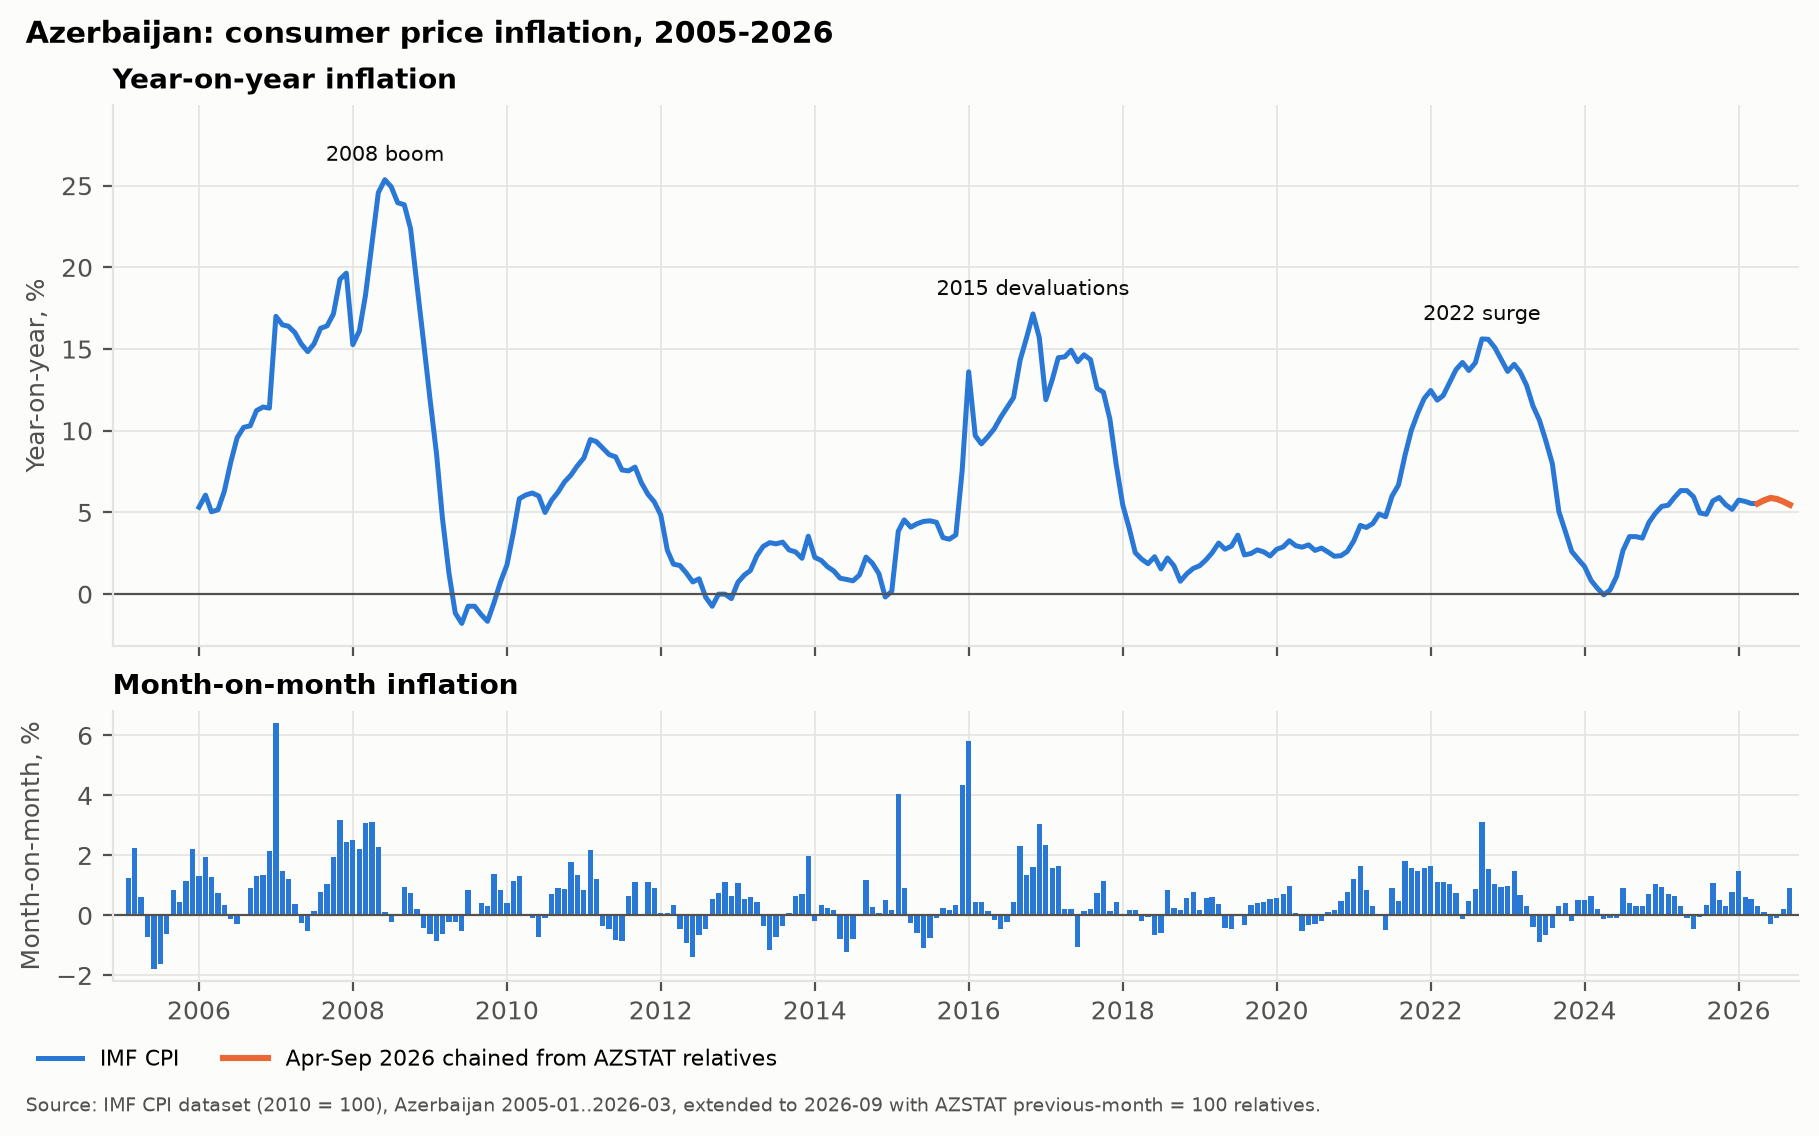
\includegraphics[width=\linewidth]{fig01_azerbaijan_inflation_history.png}
\caption{Azerbaijan's headline inflation history. Annual and monthly rates are computed from the IMF index, with April--September 2026 extended using AZSTAT monthly relatives. Episode labels provide historical context; the figure does not estimate their causes.}
\label{fig:history}
\end{figure}

The contrast across the three exposure windows is pronounced (Table~\ref{tab:exposure}). Between December 2020 and December 2023, the lowest expenditure decile's fixed basket increased in cost by 31.17\%, compared with 28.73\% for the highest decile. Their gap was 2.44 percentage points. This is the exposure that the two 2025 baskets would have had to the earlier price path. For annual-average prices in 2025 relative to 2024, the gap was 0.39 points. In the year to March 2026 it was only 0.09 points. Lower-expenditure baskets thus faced greater exposure in these comparisons, but the magnitude was strongly episode-dependent and the ordering across all ten deciles was not strictly monotonic.

\begin{table}[htbp]
\centering\small
\caption{Official Azerbaijani group basket-cost changes and gaps.}
\label{tab:exposure}
\begin{tabular}{@{}lrrrrr@{}}
\toprule
Window & National & D1 & D10 & D1$-$D10 & Rural$-$urban \\
\midrule
Dec. 2020--Dec. 2023 & 30.19 & 31.17 & 28.73 & 2.44 & 0.39 \\
Annual average 2025/2024 & 6.10 & 6.29 & 5.90 & 0.39 & 0.02 \\
Year to March 2026 & 5.93 & 5.94 & 5.84 & 0.09 & 0.01 \\
\bottomrule
\end{tabular}
\par\smallskip
\begin{minipage}{\linewidth}\footnotesize Basket changes are percentages; gaps are percentage points. D1 and D10 are the lowest and highest expenditure deciles. All calculations hold 2025 baskets fixed. The 2020--2023 comparison is counterfactual; annual-average and year-on-year windows are distinct.\end{minipage}
\end{table}

Food accounts for much of the surge-period difference. Its division price index rose by 39.97\% from December 2020 to December 2023. The exact decomposition assigns food 18.16 percentage points of the lowest decile's basket-cost increase and 11.61 points of the highest decile's increase, a difference of 6.55 points (Figure~\ref{fig:contributions}). The final gap is smaller because other categories offset part of that contribution. Furnishings contribute about 1.24 points more to the highest decile, restaurants and hotels about 0.98 points more, and transport about 0.53 points more. Exposure therefore reflects the full combination of budget shares and relative price changes. A food-share comparison alone would overstate the net gap in this episode.

\begin{figure}[htbp]
\centering
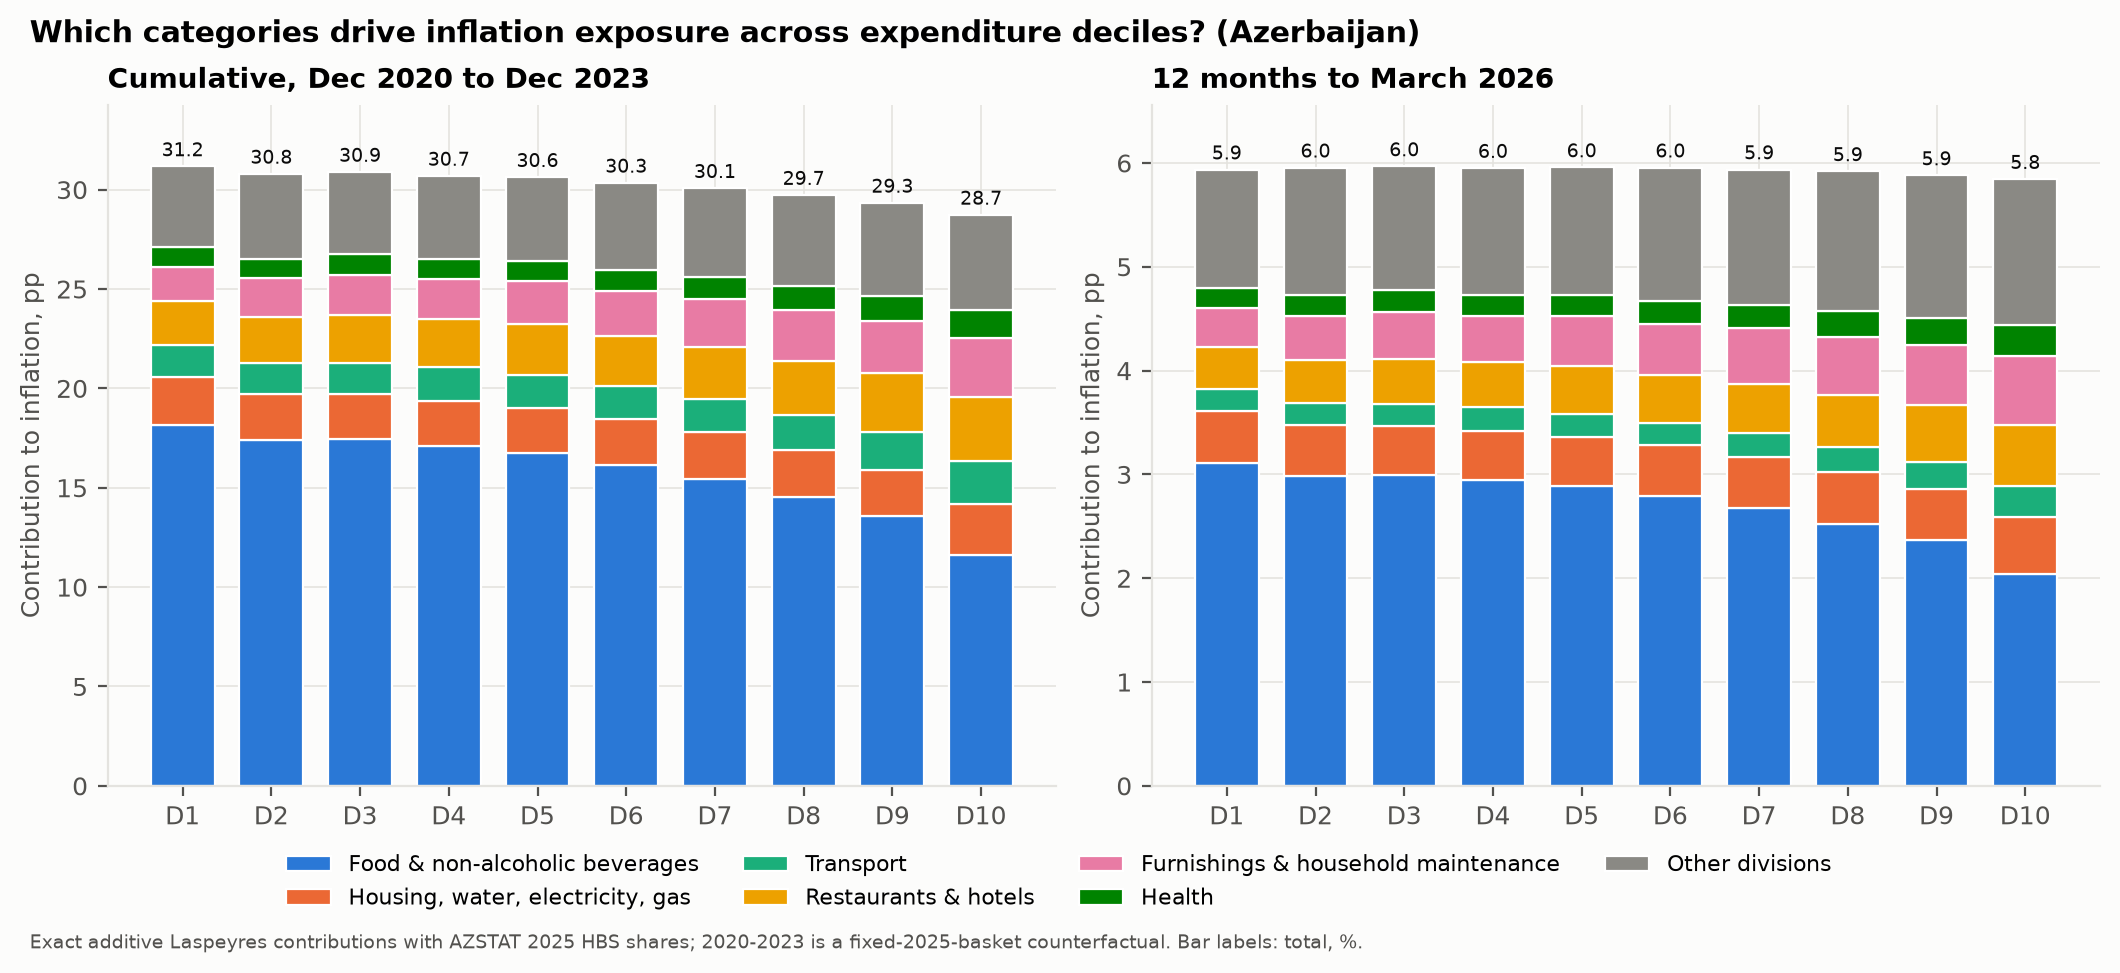
\includegraphics[width=\linewidth]{fig13_category_contributions_by_decile.png}
\caption{Category contributions to basket-cost increases across Azerbaijan's expenditure deciles. Contributions add exactly to each decile's total before rounding. The left panel is a fixed-2025-basket counterfactual for December 2020--December 2023; the right panel covers the year to March 2026.}
\label{fig:contributions}
\end{figure}

In the year to March 2026, food prices rose by approximately 6.4\%, much closer to all-items inflation of approximately 5.6\%. Although the food shares of the two deciles remained different by construction, this relative price pattern generated little net separation in their basket inflation. The national HBS-weighted estimate was 5.93\%, compared with about 5.55\% from the headline CPI series. The difference is expected because the HBS structure used here is not the official CPI weight system. National CPI inflation is consequently a benchmark for the price environment, rather than an accounting total that every constructed group estimate must reproduce.

The monthly counterfactual series makes the episode dependence clearer (Figure~\ref{fig:gap}). Over January 2006--March 2026 the lowest--highest decile gap was positive in 74.5\% of the 243 months, but it also became negative. Its association with relative food inflation has an estimated slope of 0.288, with a Newey--West 95\% interval of 0.252--0.324 and $R^2=0.857$. This is consistent with the accounting mechanism: when food rises faster than the general index, the basket with the larger food share tends to rise faster. The fit should not be interpreted as evidence that relative food inflation exogenously causes a particular change in welfare or as an independently tested forecast relationship.

\begin{figure}[htbp]
\centering
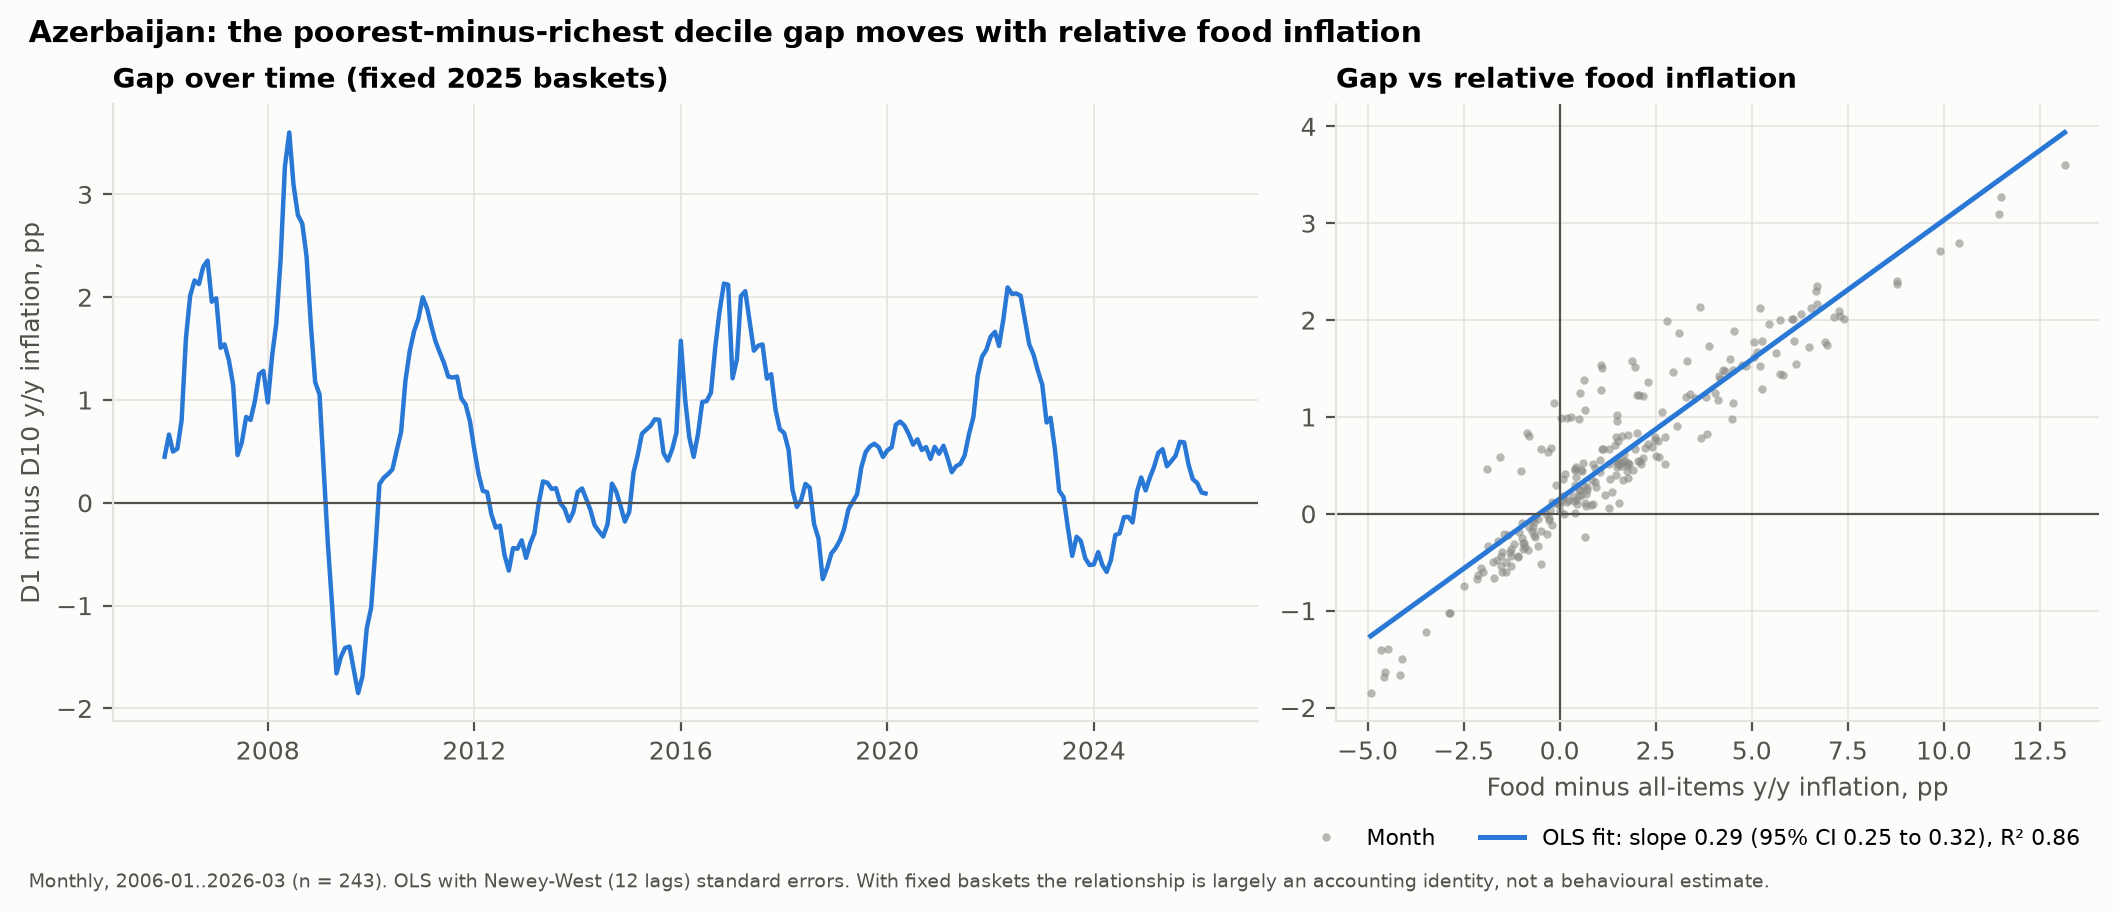
\includegraphics[width=\linewidth]{fig14_gap_vs_relative_food_inflation.png}
\caption{The lowest--highest expenditure-decile inflation gap and relative food inflation in Azerbaijan, January 2006--March 2026. All historical group observations use fixed 2025 baskets. The fitted relationship summarizes a shared-price accounting association; it is not a causal estimate. References to poorer and richer groups within the supplied graphic denote expenditure ranks.}
\label{fig:gap}
\end{figure}

The official geographical comparison is smaller. The rural-minus-urban gap was 0.39 points over the surge window and less than 0.01 points in the year to March 2026. Other official profiles, including household size, children, and the household head's education, show variation as well, but do not establish independent demographic effects. Groups overlap and share the same national division prices. Published standard errors are unavailable, so statistical significance cannot be assigned to these official differences. For the March 2026 decile gap, the central 95\% of the rounding perturbations spans 0.086--0.098 points. This narrow range establishes stability to the specified rounding exercise, without resolving sampling error or category mismatch.

The Baku pilot illustrates how household composition can differ from the national basket. In the quality-controlled sample, food at home accounts for 23.85\% of recorded spending and education for 14.01\%, compared with 42.3\% for national HBS food excluding alcohol and 1.7\% for education. The categories are not perfectly matched, and these differences also reflect the survey's selection and recall. Mean basket exposure is 5.42\% in the year to March 2026 and 26.22\% over the surge window, below the corresponding national HBS measures. Appendix~\ref{app:survey} presents the spending profiles and household distributions. These comparisons show the consequences of different reported baskets, without establishing a population pattern from the pilot.

Within the twenty-six retained households, the difference in March 2026 exposure between households below and at or above 5,000 AZN monthly income is 0.24 percentage points, with an unadjusted bootstrap 95\% interval of $-0.08$ to 0.56 points. No quality-controlled group comparison survives the specified Holm correction. The minimum detectable exposure difference at 80\% power is approximately 0.47 points, substantially larger than the official decile gap for this window. The lack of significance therefore leaves the survey evidence inconclusive. Mean exposure changes little across cleaning and mapping variants, whereas spending-to-income burdens change sharply: mean total spending is about 393\% of bracket-midpoint income in the full sample, 83\% after quality checks, and 68\% in the consistency subgroup. The reported burdens are sensitive to contradictory records and income measurement in a way that normalized basket exposure is not.

Turning to forecasting, the national comparison favors SARIMA in Azerbaijan (Table~\ref{tab:azeaccuracy} and Figure~\ref{fig:azeforecasts}). Its one-month monthly-inflation RMSE is 0.448 percentage points, compared with 0.689 for seasonal naive, 0.487 for ETS, and 0.526 for weighted fuzzy time series. SARIMA remains the lowest-RMSE primary model at three, six, and twelve months. The weighted fuzzy method improves on seasonal naive by 23.7\% at one month in point RMSE, but its bootstrap skill interval includes zero and its adjusted test is not significant ($p=0.204$). Its RMSE is higher than SARIMA's at every horizon, with within-cell adjusted differences significant at three months ($p=0.041$) and six months ($p<0.001$). SARIMA's one-month improvement over seasonal naive is marginal under the same correction ($p=0.0497$). These results do not support an accuracy advantage for the weighted fuzzy method.

\begin{table}[htbp]
\centering\small
\caption{Azerbaijan headline monthly-inflation forecast RMSE, Analysis A.}
\label{tab:azeaccuracy}
\begin{tabular}{@{}lrrrrr@{}}
\toprule
Horizon & Seasonal naive & SARIMA & ETS & Weighted fuzzy & $n$ \\
\midrule
1 & 0.689 & \textbf{0.448} & 0.487 & 0.526 & 93 \\
3 & 0.695 & \textbf{0.525} & 0.620 & 0.750 & 91 \\
6 & 0.701 & \textbf{0.531} & 0.699 & 0.845 & 88 \\
12 & 0.710 & \textbf{0.539} & 0.685 & 0.650 & 82 \\
\bottomrule
\end{tabular}
\par\smallskip
\begin{minipage}{\linewidth}\footnotesize RMSE is in percentage points of monthly inflation. Bold identifies the lowest point RMSE among the four primary models. Specifications were selected on 2016--2018 validation targets and held fixed during testing. Longer-horizon targets begin later than January 2019.\end{minipage}
\end{table}

\begin{figure}[htbp]
\centering
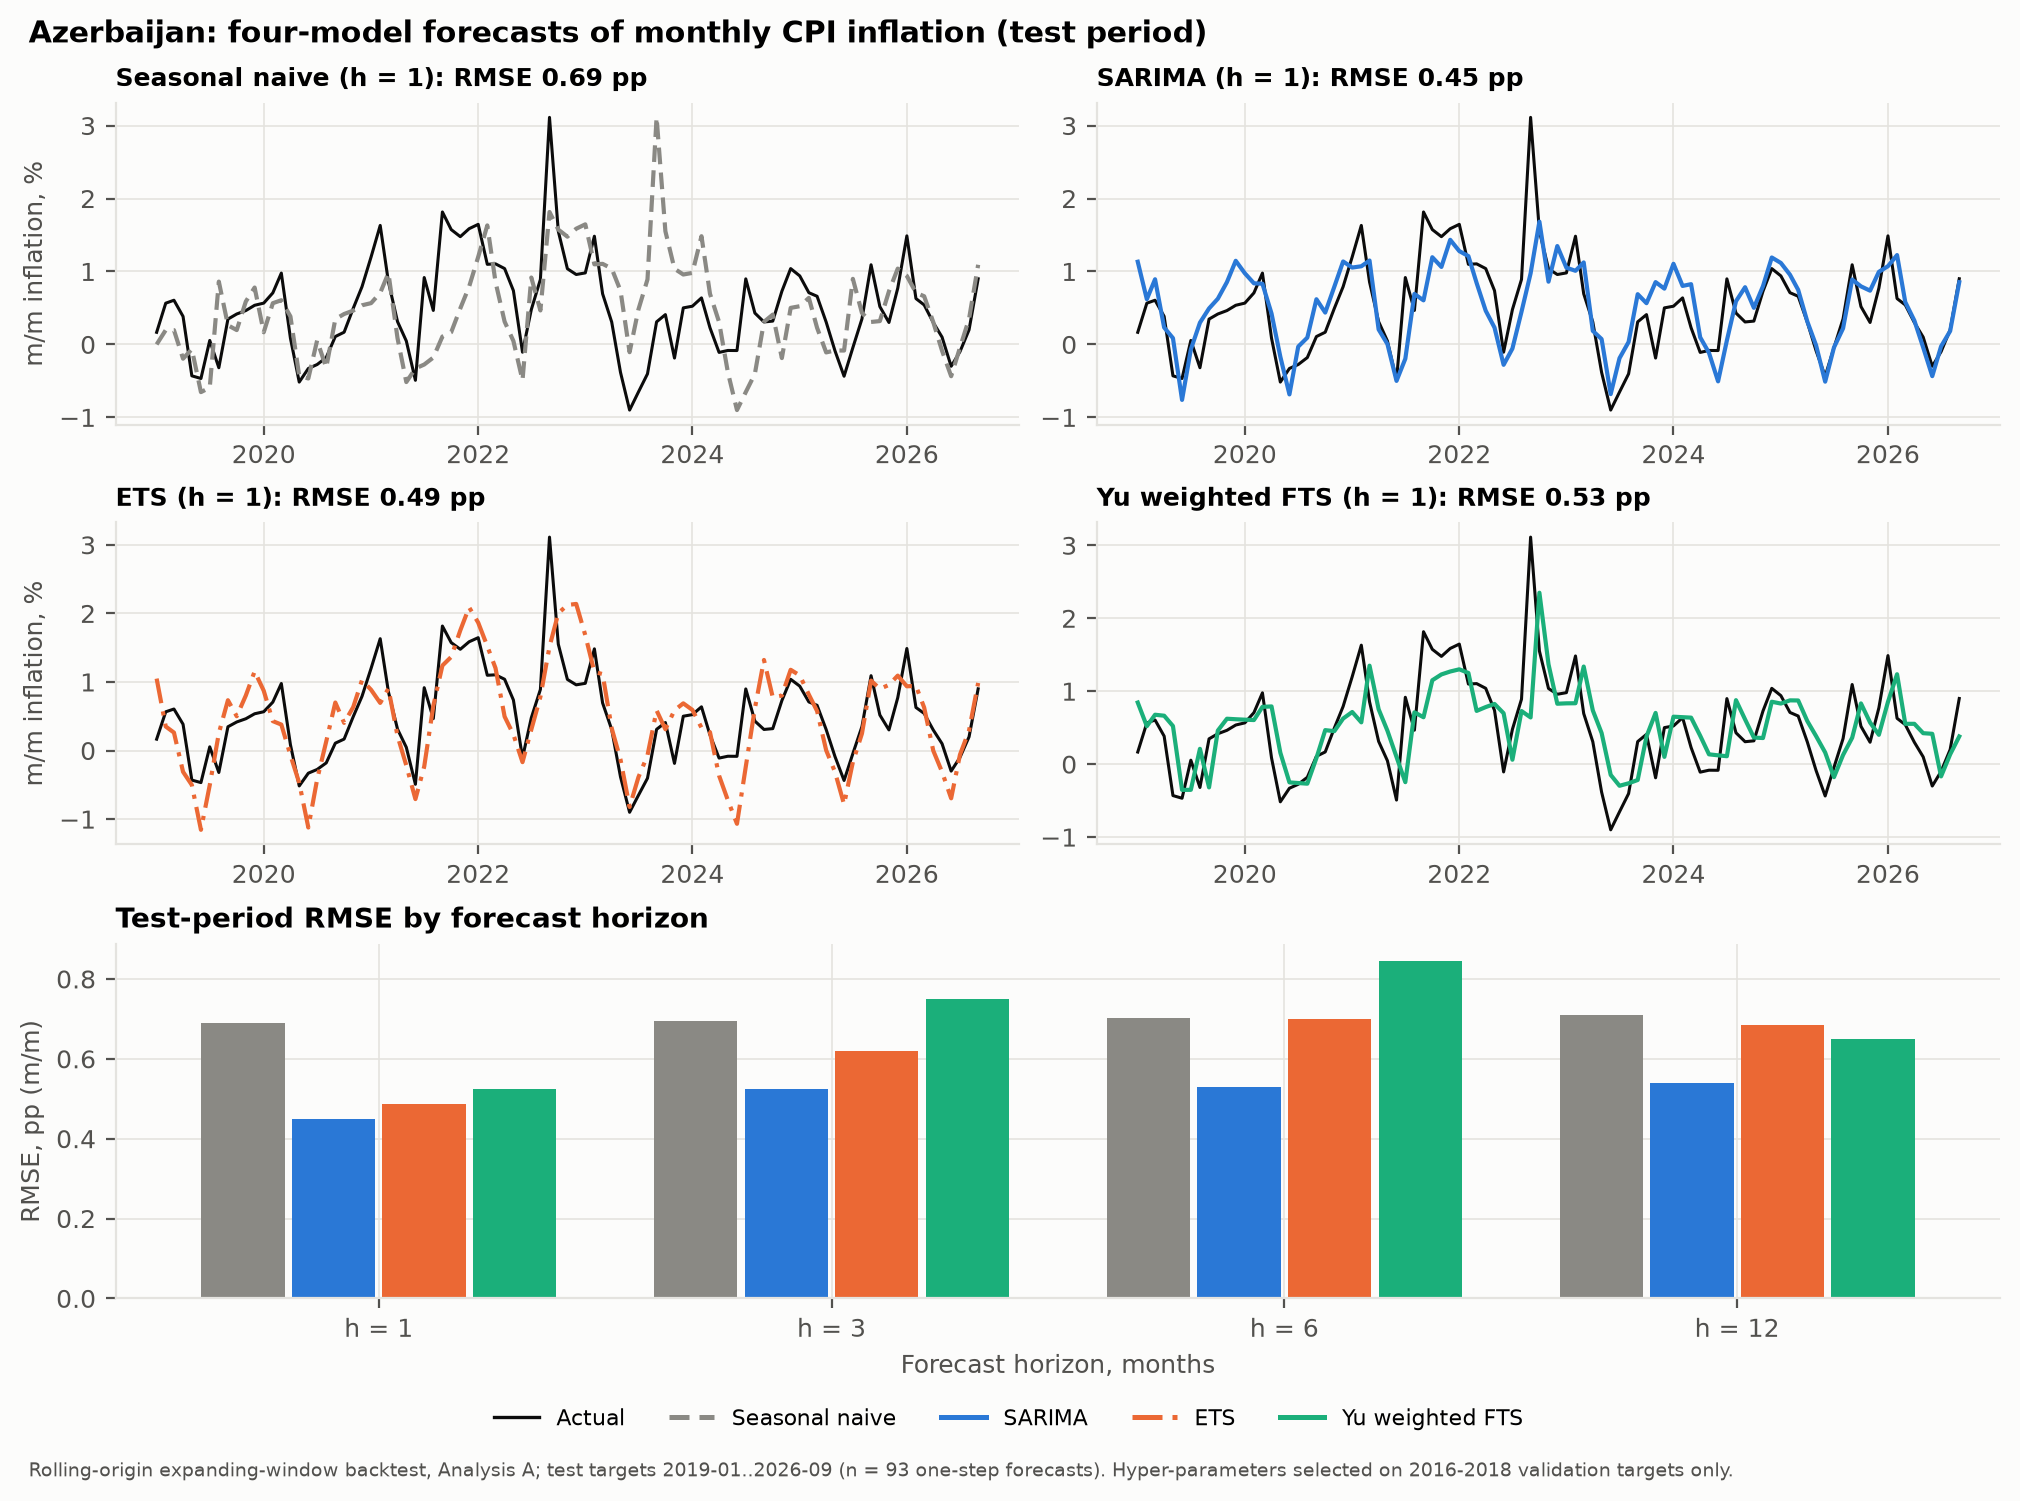
\includegraphics[width=\linewidth,height=0.57\textheight,keepaspectratio]{fig03_azerbaijan_four_model_forecasts.png}
\caption{Four-model forecasts of Azerbaijani monthly inflation in Analysis A. The line panels show rolling one-step forecasts; the lower panel compares test RMSE at the four horizons. The one-step test has 93 observations. Monthly-rate forecast errors are measured in percentage points.}
\label{fig:azeforecasts}
\end{figure}

The cross-country exercise places Azerbaijan's ranking in context (Figure~\ref{fig:skill}). Among the four primary models and twenty country--horizon cells in Analysis A, SARIMA has the lowest monthly-rate RMSE in thirteen and ETS in seven; neither seasonal naive nor weighted fuzzy time series leads a cell. The common-period exercise gives sixteen cells to SARIMA and four to ETS. These are descriptive counts across dependent comparisons. They show that the choice between the two conventional fitted models varies with country and horizon, while the fuzzy method is not the leading primary model in this sample. Appendix~\ref{app:forecast} reports the country-level one-step errors and the comparison isolating fuzzy weighting.

\begin{figure}[htbp]
\centering
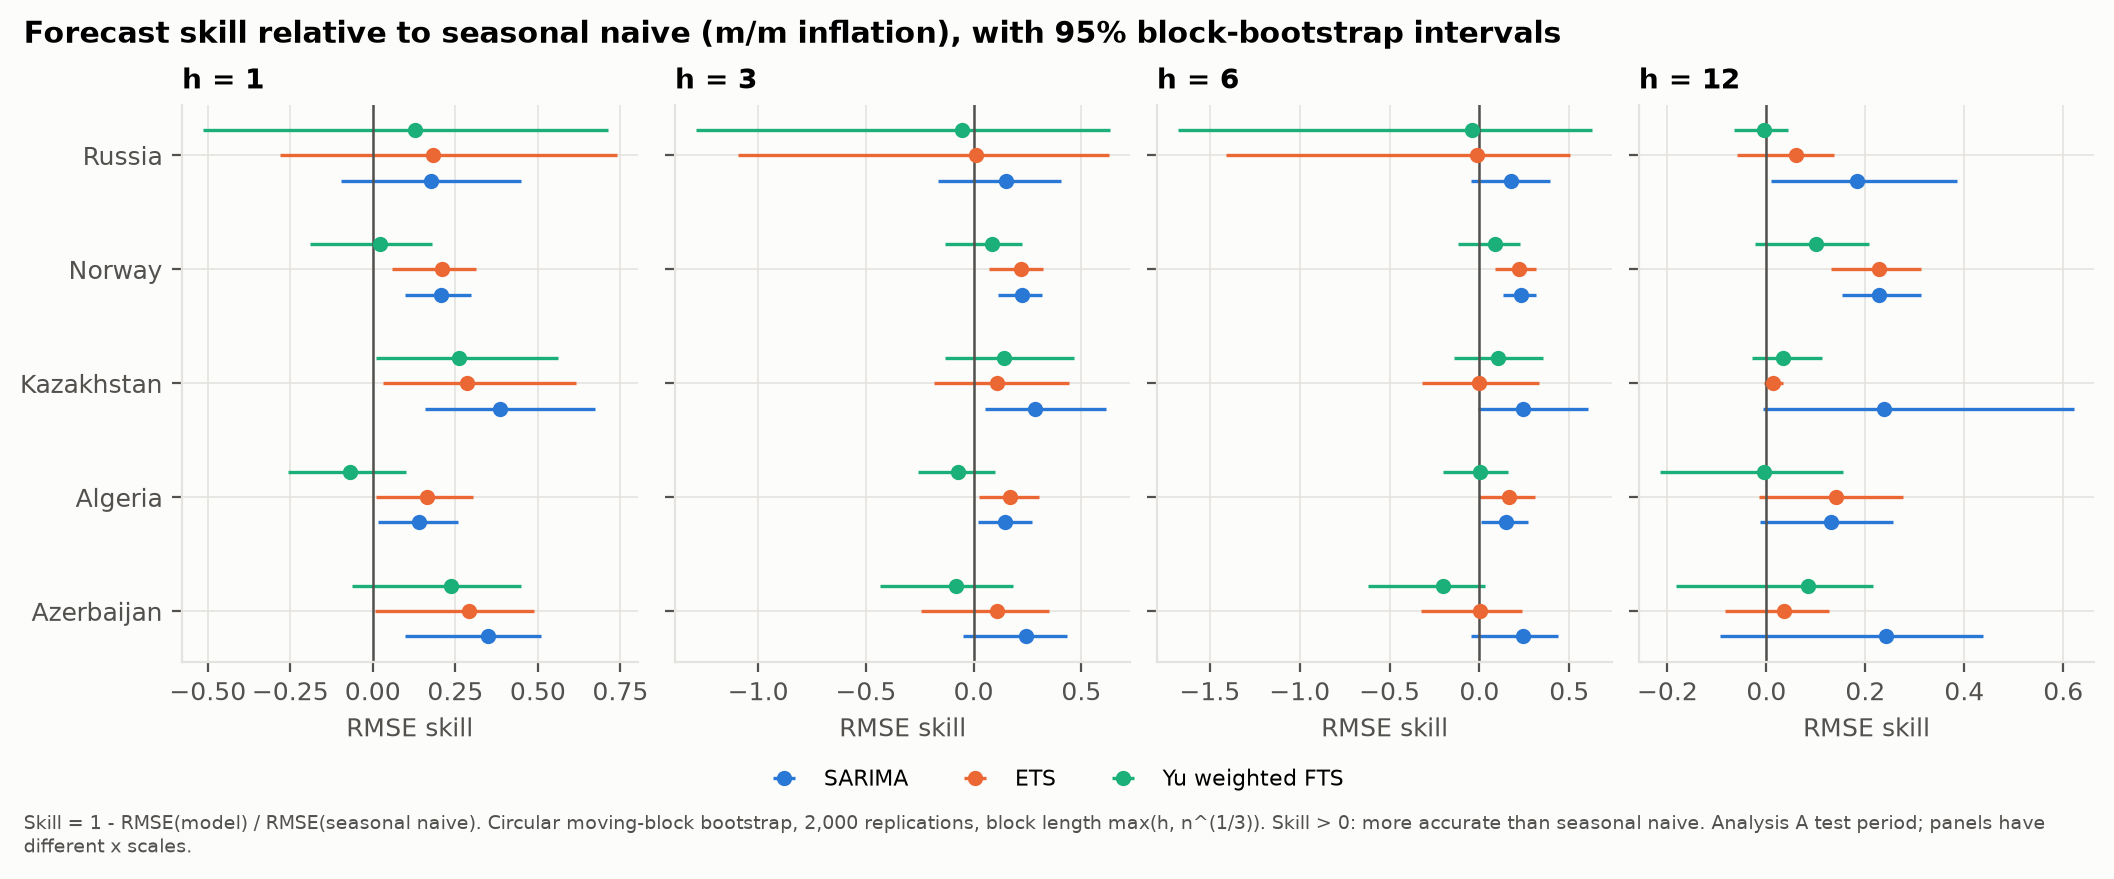
\includegraphics[width=\linewidth]{fig05_cross_country_skill.png}
\caption{Forecast skill relative to seasonal naive across the five countries, with 95\% circular moving-block bootstrap intervals. Positive skill indicates lower monthly-inflation RMSE. Horizontal scales differ between horizon panels. These intervals describe paired relative accuracy; adjusted predictive-accuracy tests are reported separately.}
\label{fig:skill}
\end{figure}

Sampling uncertainty remains material. Of 140 planned headline monthly-inflation comparisons, 27 reject after within-cell Holm adjustment; only nine reject when all 140 are treated as one family. Large apparent gains can therefore be less decisive than their point ranking suggests. Russia is a particularly clear example: the March 2022 monthly shock accounts for approximately 53\% of SARIMA's one-step squared error, and no within-cell primary comparison rejects equal predictive accuracy. A non-rejection in that setting is compatible with substantial uncertainty. Pooled common-period comparisons likewise do not show a significant advantage of weighted fuzzy time series over seasonal naive at any horizon under squared-error loss. ETS outperforms the fuzzy method in all four corresponding pooled comparisons.

The additional fuzzy comparisons narrow the interpretation further. Chronological weighting reduces RMSE relative to the equal-weight recurrence model in only nine of twenty country--horizon cells, with a median RMSE ratio of 1.005. Relative to the unique-successor model, the weighted method improves RMSE in eighteen cells, with a median ratio of 0.938. Since retaining recurrence with equal weights performs similarly, the results are consistent with recurrence being more useful than the particular recency weights. They do not establish that chronological weighting adds forecast information. The directly modelled annual-rate exercise also changes the benchmark comparison: the weighted fuzzy method has negative one-step skill relative to the annual-rate random walk in every country.

\FloatBarrier

The household forecast results bring the analysis back to its central distributional question. Across the twelve divisions and all-items series, SARIMA has the lowest RMSE among the primary models in 33 of the 52 series--horizon cells, ETS in eighteen, and weighted fuzzy time series in one. Combining the category paths with household weights produces a different forecast target from the headline monthly rate. At one month, SARIMA and ETS reduce group-inflation loss significantly relative to seasonal naive for all seven designated official groups, with within-group adjusted $p$-values no greater than 0.030. At horizons of three months or more, no primary model significantly improves on seasonal naive in those group tests. This distinction concerns the evidence for improvement; it does not mean the longer-horizon point forecasts are identical.

\begin{table}[htbp]
\centering\small
\caption{Forecast RMSE for annual group inflation and the annual decile gap.}
\label{tab:groupaccuracy}
\begin{tabular}{@{}lrrrr@{}}
\toprule
Model & $h=1$ & $h=3$ & $h=6$ & $h=12$ \\
\midrule
\multicolumn{5}{@{}l}{\textit{National HBS basket inflation}} \\
Seasonal naive & 0.795 & 1.903 & 3.393 & 5.930 \\
SARIMA & 0.504 & 1.341 & 2.459 & 4.449 \\
ETS & 0.486 & 1.248 & 2.460 & 5.066 \\
Weighted fuzzy & 0.615 & 1.958 & 3.953 & 7.826 \\
\multicolumn{5}{@{}l}{\textit{Lowest--highest decile gap}} \\
Seasonal naive & 0.155 & 0.348 & 0.611 & 1.035 \\
SARIMA & 0.108 & 0.241 & 0.408 & 0.664 \\
ETS & 0.128 & 0.339 & 0.719 & 1.318 \\
Weighted fuzzy & 0.180 & 0.567 & 1.190 & 2.048 \\
\bottomrule
\end{tabular}
\par\smallskip
\begin{minipage}{\linewidth}\footnotesize All errors are percentage points. Category data end in March 2026. Test sample sizes are 87, 85, 82, and 76 at horizons 1, 3, 6, and 12. Group targets condition on fixed 2025 basket information defined retrospectively. Gap point rankings are not significance tests.\end{minipage}
\end{table}

SARIMA has the lowest point RMSE for the lowest--highest decile gap at every horizon (Table~\ref{tab:groupaccuracy}). The gap RMSE rises from 0.108 points at one month to 0.664 points at twelve months, compared with 0.155 and 1.035 for seasonal naive and 0.180 and 2.048 for weighted fuzzy time series. These gap rankings are descriptive; the saved significance tests concern group inflation relative to seasonal naive, rather than a separate family of paired gap tests. Nevertheless, scoring the gap directly reveals a practical weakness that a headline assessment alone could miss: errors in the category paths can materially distort the projected difference between baskets.

That weakness is visible in the March 2027 scenarios computed from the March 2026 price origin (Table~\ref{tab:projections} and Figure~\ref{fig:projections}). The national HBS basket's projected annual inflation ranges from 4.20\% under ETS to 10.26\% under weighted fuzzy time series. The projected lowest--highest decile gap is positive under seasonal naive, SARIMA, and weighted fuzzy time series, but negative under ETS. Across the sixty official profiles, the projected rankings have a Spearman correlation of 0.92 between SARIMA and weighted fuzzy time series and $-0.74$ between SARIMA and ETS. These correlations compare overlapping group profiles and are descriptive. The models disagree about both the level and the ordering of exposure.

\begin{table}[htbp]
\centering\small
\caption{March 2027 annual inflation scenarios, conditional on the March 2026 price origin.}
\label{tab:projections}
\begin{tabular}{@{}lrrrrr@{}}
\toprule
Model & National & D1 & D10 & D1$-$D10 & National 80\% interval \\
\midrule
Seasonal naive & 5.95 & 5.96 & 5.87 & 0.09 & [-5.24, 13.08] \\
SARIMA & 6.63 & 6.82 & 6.33 & 0.48 & [1.19, 13.55] \\
ETS & 4.20 & 3.93 & 4.67 & -0.74 & [-3.20, 10.17] \\
Weighted fuzzy & 10.26 & 10.96 & 9.10 & 1.86 & [-0.17, 16.97] \\
\bottomrule
\end{tabular}
\par\smallskip
\begin{minipage}{\linewidth}\footnotesize Group rates and national intervals are percentages; D1$-$D10 is percentage points. These retrospective projections were computed with later basket information. Intervals use historical group forecast errors and do not include uncertainty in shares. No gap interval is inferred from the marginal bands.\end{minipage}
\end{table}

\begin{figure}[htbp]
\centering
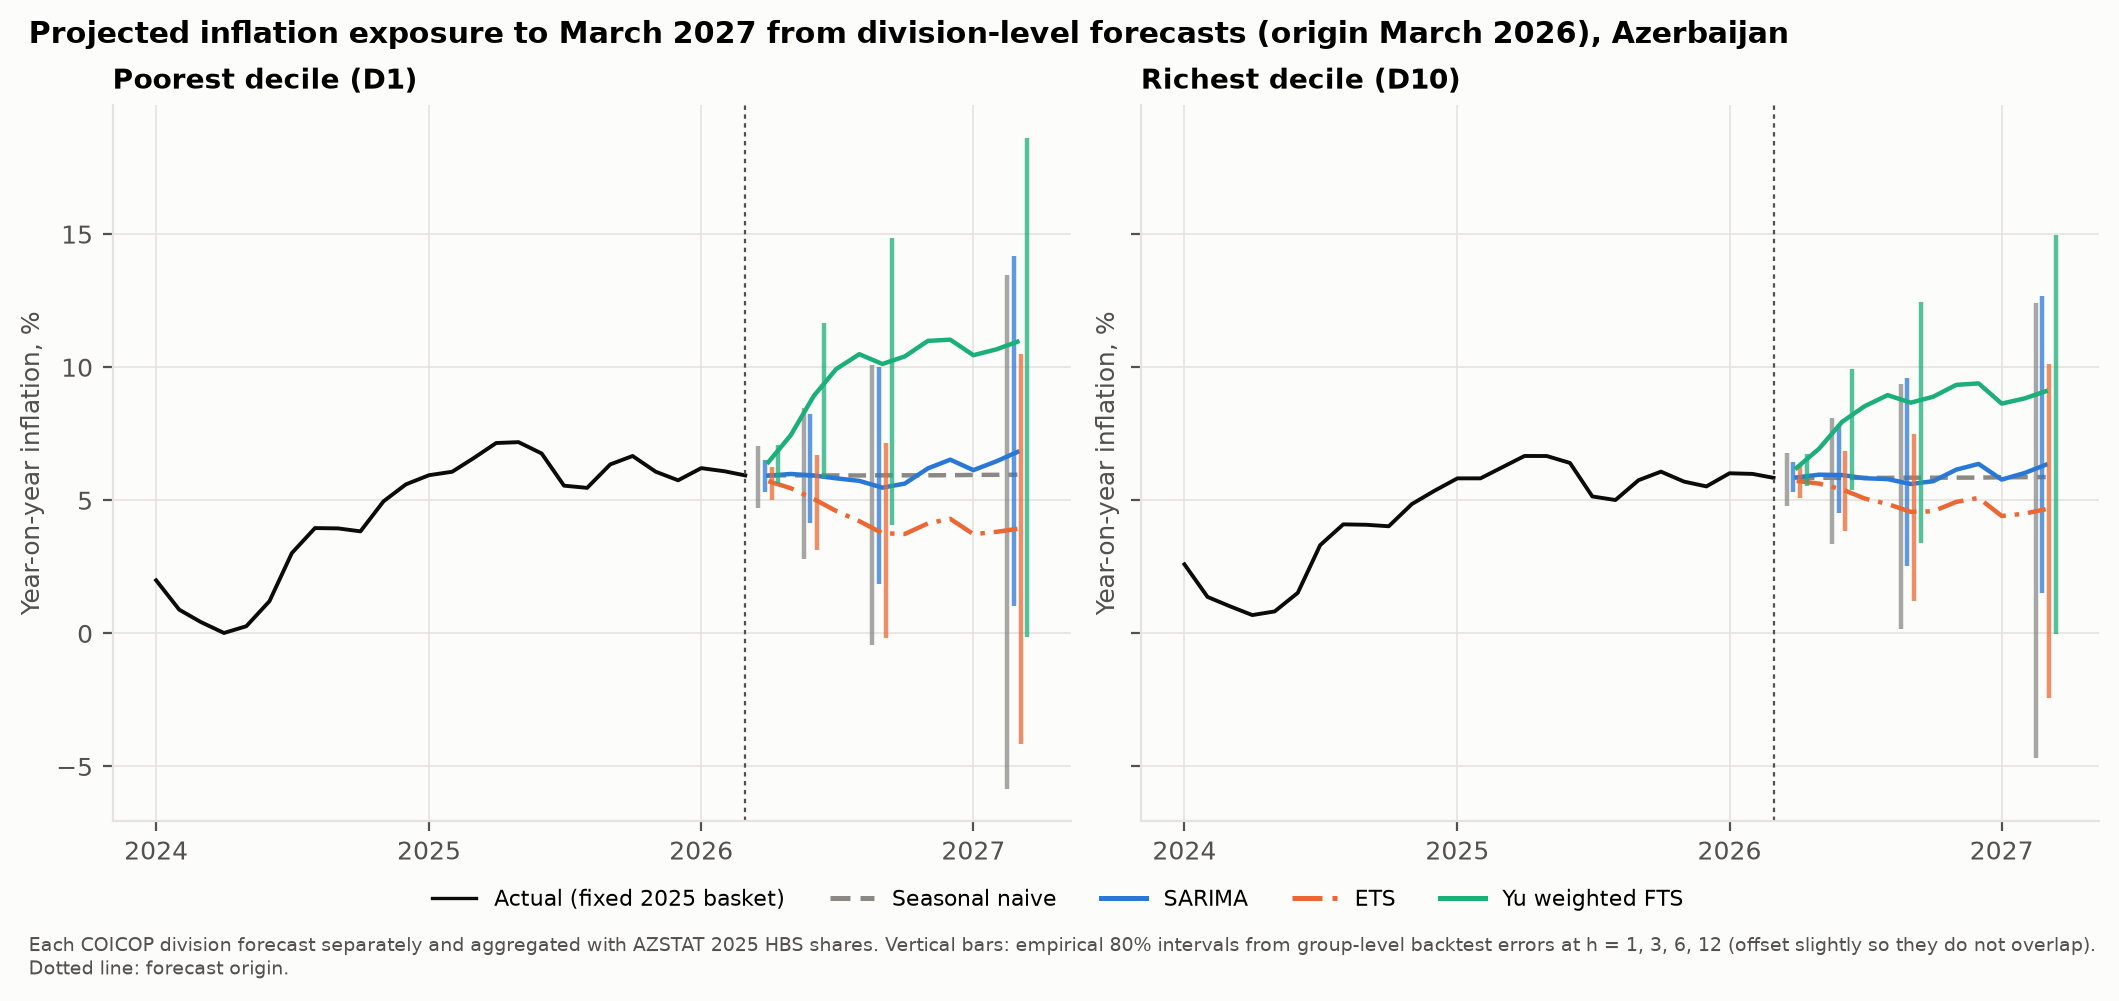
\includegraphics[width=\linewidth]{fig12_household_exposure_forecasts.png}
\caption{Retrospective scenario paths for the lowest and highest expenditure deciles, using price data through March 2026 and fixed 2025 baskets. The supplied graphic's poorer/richer labels refer to expenditure deciles. Vertical bars are empirical 80\% intervals at selected horizons, shifted slightly for visibility. These are marginal group intervals, not intervals for the difference between groups.}
\label{fig:projections}
\end{figure}

Uncertainty also appears within each model. SARIMA's empirical 80\% interval for March 2027 national-basket inflation is approximately 1.19--13.55\%. Such a range does not support a precise distributional prediction. The additional April--September 2026 check is more encouraging for short-run headline paths: the absolute annual-rate forecast error stays below 0.35 points for SARIMA and 0.34 points for seasonal naive, while ETS underpredicts by as much as 2.70 points and the weighted fuzzy method overpredicts by as much as 2.74 points. This six-observation check is retrospective, uses the stored data vintage, and assesses the all-items series only. It provides no direct observation of the household exposure gap during those months.

Kazakhstan offers an additional view of how the same basket mechanism changes across episodes. Its published food and non-alcoholic-beverage share rises from 38.6\% in 2010 to 54.2\% in 2020 and stands at 52.4\% in 2025, compared with Azerbaijan's 42.3\%. Figure~\ref{fig:baskets} compares the mapped 2025 national structures. These shares indicate different expenditure composition, without identifying differences in incomes, preferences, or household welfare from the price analysis alone.

\begin{figure}[htbp]
\centering
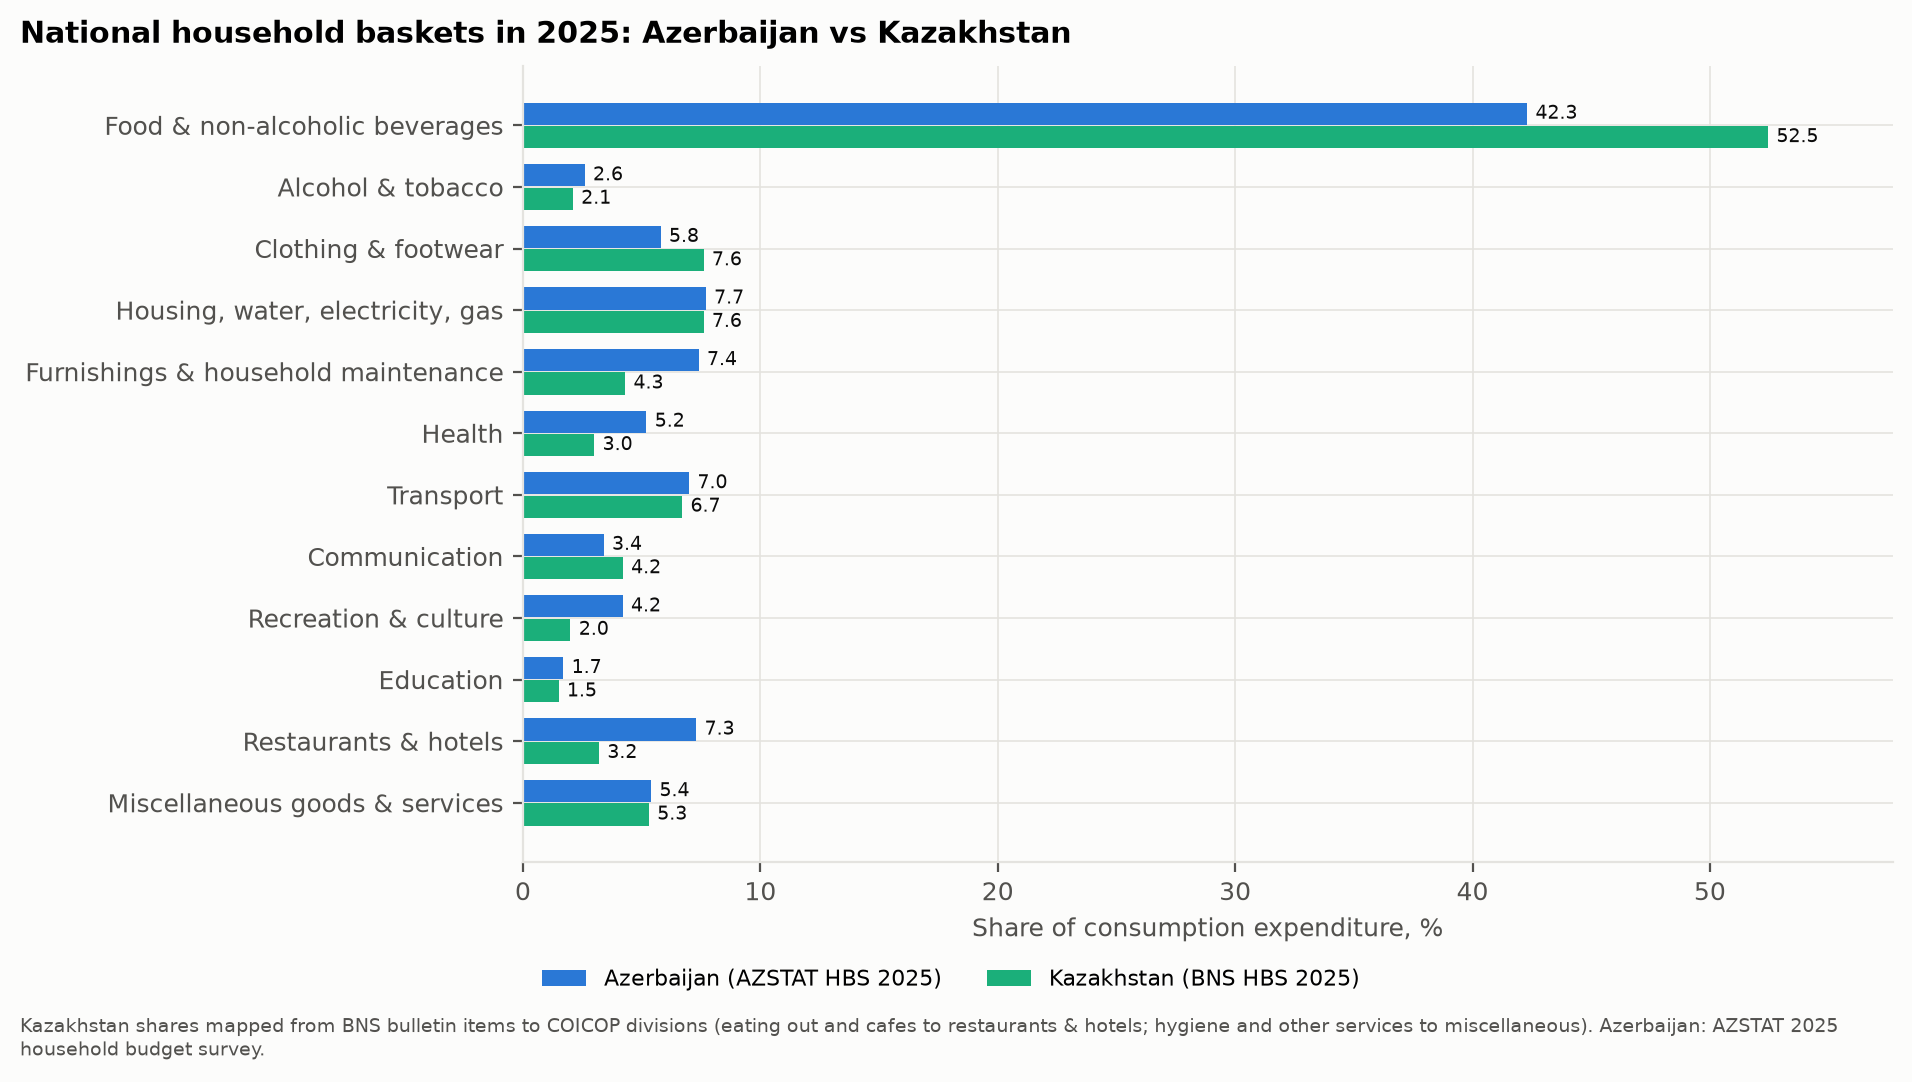
\includegraphics[width=\linewidth]{fig18_azerbaijan_kazakhstan_baskets.png}
\caption{National household expenditure baskets mapped to twelve COICOP divisions. Kazakhstan's published 2025 food share is 52.4\%; normalization of mapped components summing to 99.9\% gives 52.452\%, displayed as 52.5\% in the graphic. The national basket comparison is not an equivalence of official CPI weights.}
\label{fig:baskets}
\end{figure}

Kazakhstan's fixed-2025 national basket rises in cost by 43.36\% over December 2020--December 2023, and by 9.03\% in the year to September 2026. Across its twenty regional baskets, exposure over the surge window is positively associated with food shares (Spearman correlation 0.90). In the September 2026 annual comparison the association reverses ($-0.76$), when food inflation is below all-items inflation (Figure~\ref{fig:kazregional}). Because every region is valued at national division prices, the reversal concerns basket composition rather than regional price shocks. The rural-minus-urban annual gap remains within approximately $\pm0.34$ points over the constructed series. Supplementary figures show the consumption history and the gap's association with relative food inflation. This comparison reinforces the episode dependence of exposure without implying that Kazakhstan's geographical groups are interchangeable with Azerbaijan's expenditure deciles.

\begin{figure}[htbp]
\centering
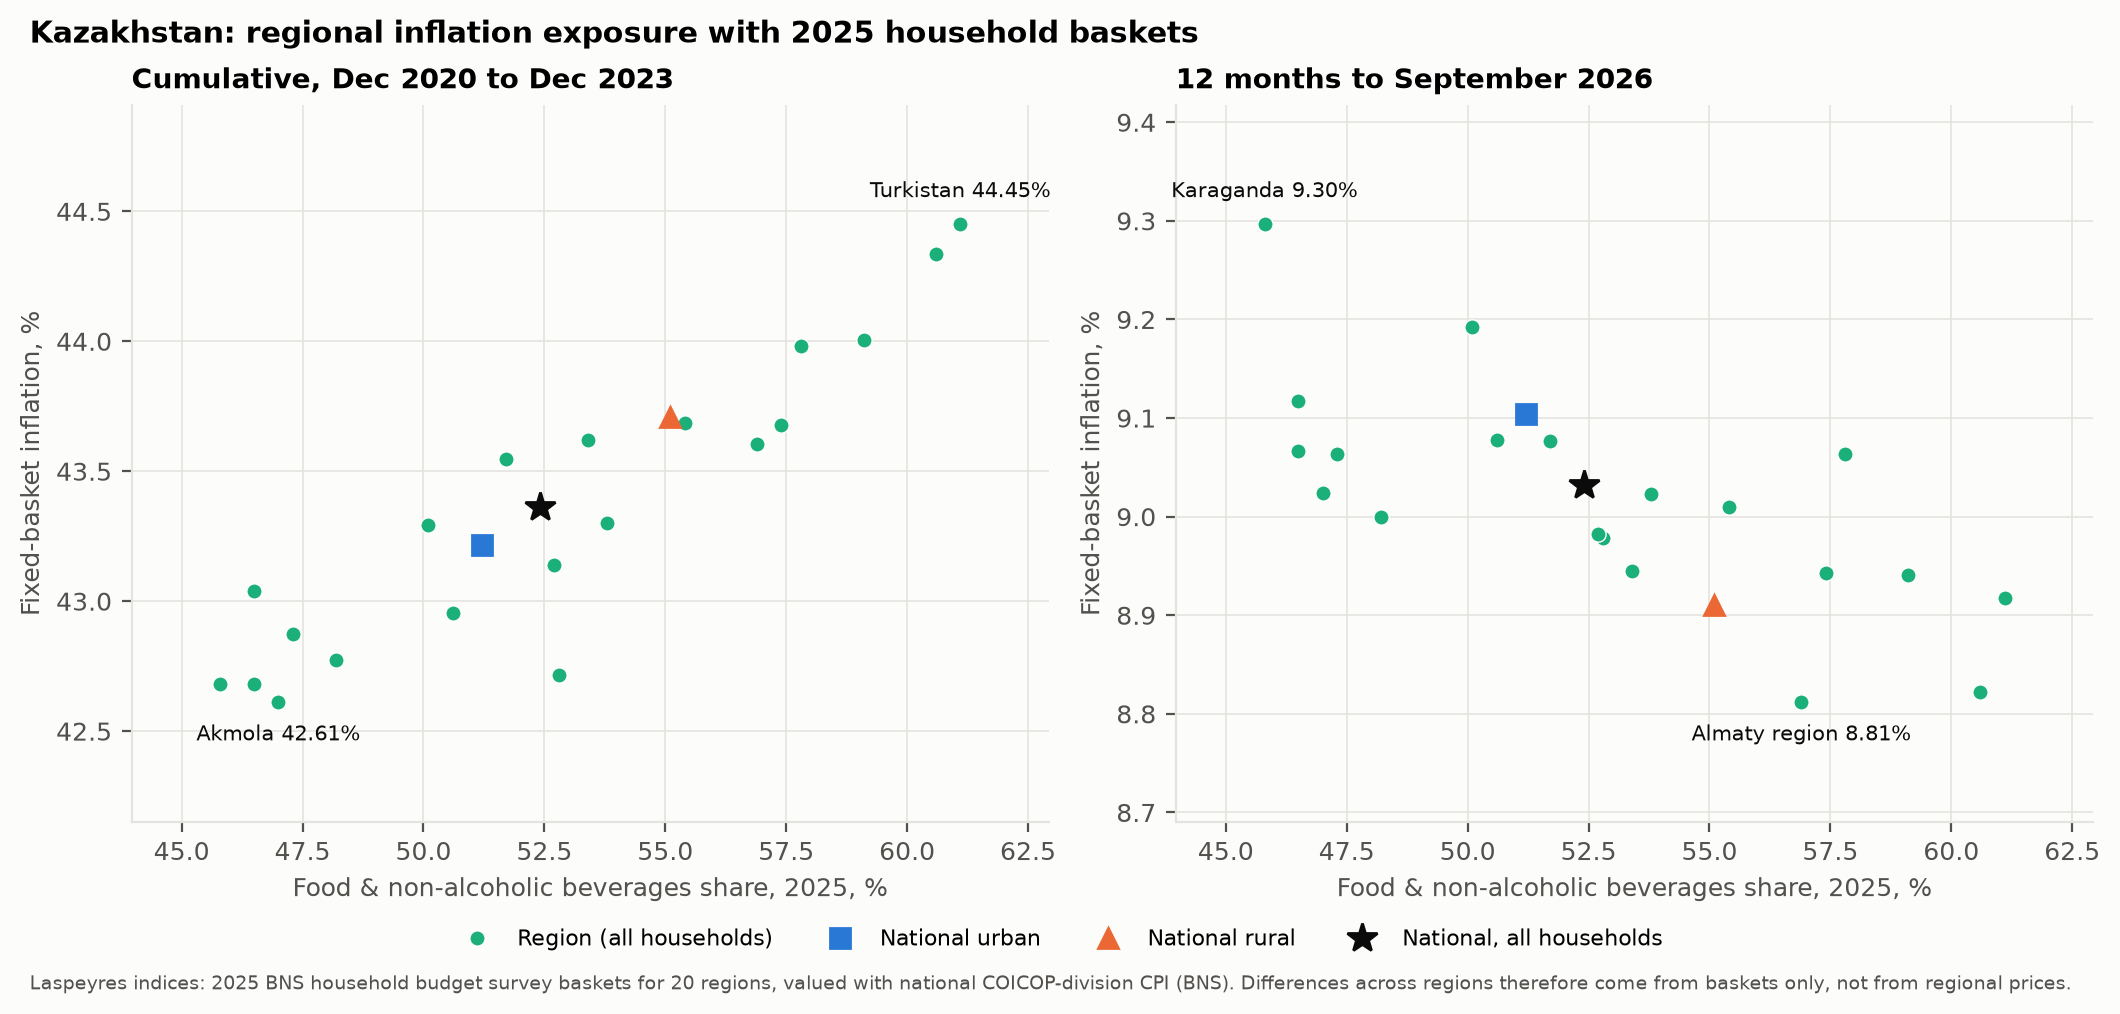
\includegraphics[width=\linewidth]{fig16_kazakhstan_regional_exposure.png}
\caption{Kazakhstan regional baskets under national division prices. The left panel values 2025 baskets over the earlier surge as a counterfactual; the right panel uses the year to September 2026. The reversal in the relationship with food shares reflects changing relative price movements. The regional points identify basket effects, not differences in prices paid across locations.}
\label{fig:kazregional}
\end{figure}

\section{Discussion and limitations}

The results give a consistent account of why inflation exposure can widen and then contract across expenditure groups. Food has a larger place in lower-expenditure Azerbaijani baskets, but that alone does not determine their inflation rate. The full relative price vector matters. During the 2020--2023 surge, food's contribution widened the decile gap substantially, while furnishings, restaurants, transport, and other categories offset part of it. In the year to March 2026 the net gap was much smaller. The variation over time is consistent with the episode-specific interpretation in \citet{lydon2022} and the budget-composition emphasis in \citet{can2025}, without requiring that all countries share the same category drivers.

The forecasting evidence adds a separate qualification. National forecast performance and household forecast performance concern related but distinct targets. SARIMA performs best in point RMSE for Azerbaijan's headline monthly rate and its decile gap, yet convincing evidence of improved group-inflation prediction relative to seasonal naive is concentrated at one month. Beyond that horizon, large uncertainty and disagreement over the direction of the projected gap weaken precise distributional claims. An operational monitoring exercise should therefore evaluate the basket differences it aims to use, alongside the aggregate rate, and show alternative category paths where rankings are unstable.

Several limits define what can be inferred. The official basket profiles are published aggregates for 2025, without the household microdata or design-based standard errors required to quantify sampling uncertainty. Exposure before that year is counterfactual. Using later baskets and their reference prices in the historical backtest also means that the evaluated target is defined with information unavailable at earlier origins. A fully real-time exercise would require historical basket vintages, their publication dates, and real-time price vintages. The present analysis isolates the forecastability of a fixed basket target conditional on its later definition.

Historical evidence on survey coverage gives an additional reason for care. \citet{ersado2006} identifies low participation by wealthy households as one explanation for unusually low measured inequality in Azerbaijan's 2002--2004 survey data. That finding concerns an earlier survey period and cannot establish the size or direction of coverage error in the 2025 baskets. It does show why published expenditure groups should not be assumed to recover the full range of household circumstances without further survey-design evidence.

The use of twelve divisions imposes further aggregation. Households within the same division may buy different goods, shop at different outlets, face different local prices, or pay different housing costs. Those differences can either widen or narrow the estimated gaps. The direction of the omitted effect is not established by the available data. Published HBS categories and price divisions also require mapping, while Kazakhstan's 2026 classification bridge and rescaling of inconsistent rural nonfood detail add construction uncertainty. Rounding perturbations and cross-source checks address particular numerical issues; they do not resolve these broader measurement questions.

The Baku survey has a different role and a different set of limitations. It is a small convenience sample, with a pronounced concentration of higher-income households and no rural respondents. Its October 2026 spending is treated as a fixed reference basket alongside the 2025 official data. Bracketed income, recall of irregular purchases, and contradictory reported totals affect burden measures in particular. Quality checks and alternative category mappings expose this sensitivity, but cannot make the sample representative. Household-level null findings consequently provide little evidence about the absence of population differences.

Forecast conclusions are conditional on the implemented model classes, limited selection grids, and one validation period. The study does not compare every nonlinear method or use external predictors such as exchange rates, import prices, administered-price announcements, or wages. Univariate methods cannot anticipate shocks that are absent from their information set. Some residual diagnostics indicate remaining serial dependence or non-normality, and recursive fuzzy forecasts can remain in a state associated with an unprecedented shock. The evidence is therefore about these specified methods, rather than a general verdict on every fuzzy or nonlinear model.

Inference is also constrained by short test sequences, overlapping multi-step errors, and extreme observations. The forecast tests use a horizon-based long-run variance truncation, which may not capture all remaining dependence. The reduction from 27 within-cell rejections to nine under global adjustment shows why individual significant comparisons should not be generalized casually. Interval calibration varies: model-based 80\% intervals tend to overcover, while empirical intervals under-cover at longer horizons in the headline experiments. Projection intervals based on past errors cannot guarantee protection against a new shock, and marginal group intervals do not supply a calibrated interval for their difference.

Finally, the analysis does not estimate welfare losses or the incidence of compensation policies. A basket-cost increase says how much more a fixed reference composition costs. Its burden on living standards also depends on income changes, transfers, savings, debt, substitution possibilities, and the household's initial circumstances. The findings can identify categories and baskets worth monitoring, but do not by themselves establish an optimal transfer schedule or rank households by welfare damage. Their practical contribution is a transparent account of measured exposure and a direct test of how uncertain its forecasts remain.

\section{Conclusion}

Inflation exposure across Azerbaijani expenditure groups varies with the composition of price changes. Applying official 2025 baskets to the 2020--2023 surge gives a lowest--highest decile gap of 2.44 percentage points, compared with 0.09 points in the year to March 2026. Food explains much of the surge-period separation, while other categories offset part of it. The Kazakhstan extension similarly shows that the relationship between food shares and exposure can reverse across episodes.

Forecast evaluation yields a more qualified conclusion. SARIMA is the strongest primary model in point RMSE for Azerbaijan's aggregate monthly inflation and its decile gap. The weighted fuzzy method provides a useful test of recurrent states and recency weighting, but does not outperform the conventional models in this application. Statistically supported improvements in household-group inflation are concentrated at one month, and longer-horizon scenario rankings depend on model choice. Connecting category-level price measurement to explicit group and gap evaluation therefore improves the information available for household inflation monitoring, while keeping forecast uncertainty visible.

\clearpage
\section*{Author contributions}

\noindent\textbf{Youssef El Haroun --- Lead researcher, methodology and statistical modeling.} Developed the research framework and methodology, collected and organized Azerbaijan's inflation and socioeconomic datasets, and designed and implemented the statistical and inflation forecasting models. Conducted model validation, comparative analysis, and interpretation of results, and coordinated the integration of the data analysis and research findings.

\noindent\textbf{Mukhammed --- International data collection and manuscript development.} Collected inflation and economic datasets for the comparative countries and organized them for cross-country analysis. Drafted and structured manuscript sections, organized references, tables, and supporting research documentation, and edited the manuscript for academic clarity and consistency.

\noindent\textbf{Vahid Musayev --- Data quality assurance and research validation.} Verified the accuracy and reliability of collected datasets and statistical sources, checked definitions, units, and time periods across countries, and identified missing values, inconsistencies, and data limitations. Supported harmonization and reviewed the reproducibility and documentation of data preparation.

\noindent\textbf{Murad Ismayilov --- Research mentor, academic coordinator and critical reviewer; master's student, Stanford University.} Provided academic mentorship and methodological guidance, coordinated research progress, and advised on analytical approaches. Critically reviewed statistical methods, findings, and limitations, evaluated the manuscript's academic rigor and coherence, and recommended improvements to the final paper.

\section*{Data and reproducibility}

Official source data are available from AZSTAT, the IMF, the World Bank, and Kazakhstan's BNS, as identified in the references. The accompanying local research archive contains source inventories, retrieval metadata, preparation scripts, saved rolling forecasts, numerical checks, and software versions. It retains the data vintage used here rather than silently substituting revised observations. The pilot survey has no population weights; detailed household records are excluded from the manuscript upload package to reduce disclosure risk. The manuscript tables report aggregate summaries and the selected forecasts needed to evaluate the claims. No public repository or unrestricted access to survey microdata is asserted.

\clearpage
\begin{thebibliography}{99}
\footnotesize\raggedright
\setlength{\bibsep}{2pt}
\bibitem[Kazakhstan Bureau of National Statistics(2026)]{bns2026}
Bureau of National Statistics of the Agency for Strategic Planning and Reforms of the Republic of Kazakhstan (2026).
\emph{Expenses and incomes of the population}, annual bulletins 2010--2025 and first and second quarters 2026; monthly CPI by main sections.
Stored bulletins and price tables assembled 25 October 2026.
\url{https://stat.gov.kz/en/industries/labor-and-income/stat-life/};
division price table: \url{https://stat.gov.kz/api/iblock/element/1550/file/ru/}.

\bibitem[Can et~al.(2025)]{can2025}
Can, Z.~G., O'Donoghue, C., Sologon, D.~M., Smith, D., and Murray, U. (2025).
Modelling the distributional effects of the cost-of-living crisis in Turkey and the South Caucasus: A microsimulation analysis.
\emph{International Journal of Microsimulation}, 18(3), 26--49.
\href{https://doi.org/10.34196/ijm.00325}{doi:10.34196/ijm.00325}.

\bibitem[Chen(1996)]{chen1996}
Chen, S.-M. (1996). Forecasting enrollments based on fuzzy time series.
\emph{Fuzzy Sets and Systems}, 81(3), 311--319.
\href{https://doi.org/10.1016/0165-0114(95)00220-0}{doi:10.1016/0165-0114(95)00220-0}.

\bibitem[Diebold and Mariano(1995)]{diebold1995}
Diebold, F.~X., and Mariano, R.~S. (1995). Comparing predictive accuracy.
\emph{Journal of Business \& Economic Statistics}, 13(3), 253--263.
\href{https://doi.org/10.1080/07350015.1995.10524599}{doi:10.1080/07350015.1995.10524599}.

\bibitem[Ersado(2006)]{ersado2006}
Ersado, L. (2006). Azerbaijan's household survey data: Explaining why inequality is so low.
\emph{World Bank Policy Research Working Paper}, No.~4009.
\url{https://documents.worldbank.org/curated/en/117911468221371795/pdf/wps40090BOX0B311113.pdf}.

\bibitem[Harvey et~al.(1997)]{harvey1997}
Harvey, D., Leybourne, S., and Newbold, P. (1997).
Testing the equality of prediction mean squared errors.
\emph{International Journal of Forecasting}, 13(2), 281--291.
\href{https://doi.org/10.1016/S0169-2070(96)00719-4}{doi:10.1016/S0169-2070(96)00719-4}.

\bibitem[Holm(1979)]{holm1979}
Holm, S. (1979). A simple sequentially rejective multiple test procedure.
\emph{Scandinavian Journal of Statistics}, 6(2), 65--70.
\url{https://www.jstor.org/stable/4615733}.

\bibitem[Huarng(2001)]{huarng2001}
Huarng, K. (2001). Effective lengths of intervals to improve forecasting in fuzzy time series.
\emph{Fuzzy Sets and Systems}, 123(3), 387--394.
\href{https://doi.org/10.1016/S0165-0114(00)00057-9}{doi:10.1016/S0165-0114(00)00057-9}.

\bibitem[Hyndman and Athanasopoulos(2021)]{hyndman2021}
Hyndman, R.~J., and Athanasopoulos, G. (2021).
\emph{Forecasting: Principles and Practice}, 3rd edition. OTexts, Melbourne.
\url{https://otexts.com/fpp3/}. Online edition consulted 25 October 2026.

\bibitem[Hyndman and Koehler(2006)]{hyndman2006}
Hyndman, R.~J., and Koehler, A.~B. (2006). Another look at measures of forecast accuracy.
\emph{International Journal of Forecasting}, 22(4), 679--688.
\href{https://doi.org/10.1016/j.ijforecast.2006.03.001}{doi:10.1016/j.ijforecast.2006.03.001}.

\bibitem[International Monetary Fund(2026)]{imf2026}
International Monetary Fund (2026). \emph{Consumer Price Index (CPI)}, IMF.STA:CPI.
Monthly national all-items and division indices; stored data retrieved 24 October 2026.
\url{https://data.imf.org/en/datasets/IMF.STA:CPI}.

\bibitem[Lokshin et~al.(2025)]{lokshin2025}
Lokshin, M., Sajaia, Z., and Torre, I. (2025).
Who suffers the most from the cost of living crisis?
\emph{Review of Income and Wealth}, 71(1), e70009.
\href{https://doi.org/10.1111/roiw.70009}{doi:10.1111/roiw.70009}.

\bibitem[Lydon(2022)]{lydon2022}
Lydon, R. (2022). Household characteristics, Irish inflation and the cost of living.
\emph{Central Bank of Ireland Economic Letter}, Vol.~2022, No.~1.
\url{https://www.centralbank.ie/docs/default-source/publications/economic-letters/household-characteristics-irish-inflation-and-the-cost-of-living.pdf}.

\bibitem[State Statistical Committee of Azerbaijan(2026a)]{azstat2026}
State Statistical Committee of the Republic of Azerbaijan (2026a).
\emph{Results of the Household Budget Survey} [statistical yearbook in Azerbaijani], statistical yearbook, Baku.
Tables of 2025 consumption expenditure structures, including Table~37, p.~48, and Table~61, p.~72.
\url{https://www.stat.gov.az/menu/6/statistical_yearbooks/source/evtes_2026.pdf}.

\bibitem[State Statistical Committee of Azerbaijan(2026b)]{azprices2026}
State Statistical Committee of the Republic of Azerbaijan (2026b).
\emph{Prices and Price Indices}, September 2026 bulletin, with earlier monthly bulletins and annual price tables in the stored source archive.
\url{https://www.stat.gov.az/source/price_tarif/az/B/2026/Qiymetler_ve_qiymet_indeksleri_bulleten_2026_sentyabr.pdf}.

\bibitem[Walewski and Chubrik(2010)]{walewski2010}
Walewski, M., and Chubrik, A. (2010).
Oil-led economic growth and the distribution of real household incomes and consumption in Azerbaijan.
\emph{CASE Network Studies \& Analyses}, No.~417.
\href{https://doi.org/10.2139/ssrn.1713099}{doi:10.2139/ssrn.1713099}.

\bibitem[World Bank(2026)]{worldbank2026}
World Bank (2026). \emph{World Development Indicators}: Consumer price index (2010 = 100), FP.CPI.TOTL, and inflation, consumer prices (annual \%), FP.CPI.TOTL.ZG.
Stored vintage retrieved 24 October 2026.
\url{https://data.worldbank.org/indicator/FP.CPI.TOTL.ZG}.

\bibitem[Yu(2005)]{yu2005}
Yu, H.-K. (2005). Weighted fuzzy time series models for TAIEX forecasting.
\emph{Physica A: Statistical Mechanics and its Applications}, 349(3--4), 609--624.
\href{https://doi.org/10.1016/j.physa.2004.11.006}{doi:10.1016/j.physa.2004.11.006}.
\end{thebibliography}

\clearpage
\appendix
\section{Data construction and model diagnostics}
\label{app:construction}

For Azerbaijan, the published national food total is 42.9\%, including a separately identified alcohol share of 0.6\%. Removing alcohol gives CP01 at 42.3\%; combining alcohol with tobacco gives CP02 at 2.6\%. For expenditure deciles D1 and D10, the same subtraction is $48.9-0.4=48.5$ and $32.3-0.6=31.7$. Other published items map to clothing and footwear, housing-related costs, furnishings, health, transport, communication, recreation, education, restaurants and hotels, and miscellaneous goods and services. Shares are divided by their mapped total before index construction. Annual-average changes use averages of index levels, not averages of monthly inflation rates.

The survey's direct mappings follow these divisions where possible. Rent and repairs and utilities both map to CP04. Hygiene and household goods are split equally between CP05 and CP12. Family events and gifts and other consumption are assigned the all-items price index as proxies. Gifts may include transfers rather than purchases, so excluding gifts is an additional sensitivity check. Mapping hygiene entirely to either division, or dropping gifts, moves mean March 2026 exposure across approximately 5.37--5.46\%. The calculation describes spending reported in October 2026 under a fixed 2025 price normalization, rather than an observed 2025 survey basket.

The quality rules exclude duplicate submissions, negative values, straight-lining across all spending categories, an itemized total inconsistent with the respondent's stated total-spending bracket by more than a factor of two, and a spending bracket at least six bands above the income bracket. Six records fail at least one exclusion rule. Contradictory children and household-size answers are set missing for the affected demographic comparisons. Spending above reported income alone is not an exclusion: households can finance spending from savings, borrowing, or transfers. The consistency subgroup is a sensitivity restriction and is not assumed to be the uniquely correct sample.

Kazakhstan's 2025 detailed rural nonfood components do not reconcile with the corresponding summary table, with a maximum discrepancy of 2.7 percentage points. Their internal composition is rescaled to match that summary. One missing alcohol-and-tobacco monthly CPI cell, February 2014, is recovered from the year-to-date block. The mapped national 2025 division shares total 99.9\% before normalization. These adjustments are documented rather than treated as original published values. Quarterly 2026 budget structures are displayed separately from annual observations, and the 2026 COICOP change makes the price bridge approximate.

For fuzzy forecasting, the two interval-length alternatives are evaluated on validation targets only. The average-based rule rounds half the mean absolute first difference down to a scale base; the distribution-based rule uses the largest admissible multiple of a base smaller than at least half the absolute first differences. The base is extended to inflation scales using $10^{\lceil\log_{10} L\rceil-1}$, with numerical tolerance at exact powers of ten. The universe begins at a rounded value below the observed minimum and is extended to contain the maximum. Boundary observations are assigned to the nearest end interval if necessary. The model's worked-example check reproduces the forecast 3440 from midpoints $(3350,3650,3450,3350)$ and normalized weights $(1,2,3,4)/10$ \citep{yu2005}. This verifies the weighting arithmetic and recurrence, without replicating the original stock-index accuracy table.

The selected Azerbaijan headline monthly-rate specifications are SARIMA$(0,0,1)(1,0,1)_{12}$ with a constant, ETS with additive errors, a damped additive trend and additive annual seasonality, and weighted fuzzy time series with the average-based interval rule. Diagnostic evidence from the pre-test history supports annual seasonality, but stationarity evidence is mixed for some countries. Azerbaijan's monthly inflation has an augmented Dickey--Fuller $p$-value of approximately 0.057, while KPSS does not reject stationarity at 10\%. Selected SARIMA monthly-rate residuals do not reject white noise in Azerbaijan, Kazakhstan, and Norway, but remaining autocorrelation appears for Russia at lag twelve and Algeria at lag twenty-four. These findings qualify the adequacy of the fitted specifications.

All four primary methods are univariate. Model-based prediction intervals are available for SARIMA and ETS. Empirical intervals add quantiles of each method's prior errors at the same horizon and require at least twenty-four errors. In rolling evaluation, only errors with realized targets by the origin enter the interval calculation. Final March 2026 group scenarios use the realized historical errors available in the stored experiment through that price origin. These bands condition on fixed shares and omit HBS sampling uncertainty. There is no independently calibrated interval for the decile gap in the supplied outputs.

\section{Supplementary forecast evidence}
\label{app:forecast}

The five-country paths in Figure~\ref{fig:international} show why country-specific evaluation is useful. The international comparison uses rate changes to avoid confusing different index reference years. Table~\ref{tab:countryaccuracy} reports one-month point errors. These figures concern the maximum-coverage experiment; the common-period exercise fixes both training start and final evaluation month.

\begin{table}[htbp]
\centering\small
\caption{One-month headline monthly-inflation RMSE across countries, Analysis A.}
\label{tab:countryaccuracy}
\begin{tabular}{@{}lrrrrr@{}}
\toprule
Country & Seasonal naive & SARIMA & ETS & Weighted fuzzy & $n$ \\
\midrule
Azerbaijan & 0.689 & 0.448 & 0.487 & 0.526 & 93 \\
Algeria & 0.973 & 0.836 & 0.813 & 1.039 & 92 \\
Kazakhstan & 0.629 & 0.387 & 0.450 & 0.466 & 93 \\
Norway & 0.557 & 0.443 & 0.440 & 0.545 & 93 \\
Russia & 1.150 & 0.949 & 0.941 & 1.002 & 92 \\
\bottomrule
\end{tabular}
\par\smallskip
\begin{minipage}{\linewidth}\footnotesize RMSE is in percentage points. One-step targets run from January 2019 to September 2026 for Azerbaijan, Kazakhstan, and Norway, and to August 2026 for Algeria and Russia. Country differences in RMSE also reflect different inflation volatility.\end{minipage}
\end{table}

\begin{figure}[htbp]
\centering
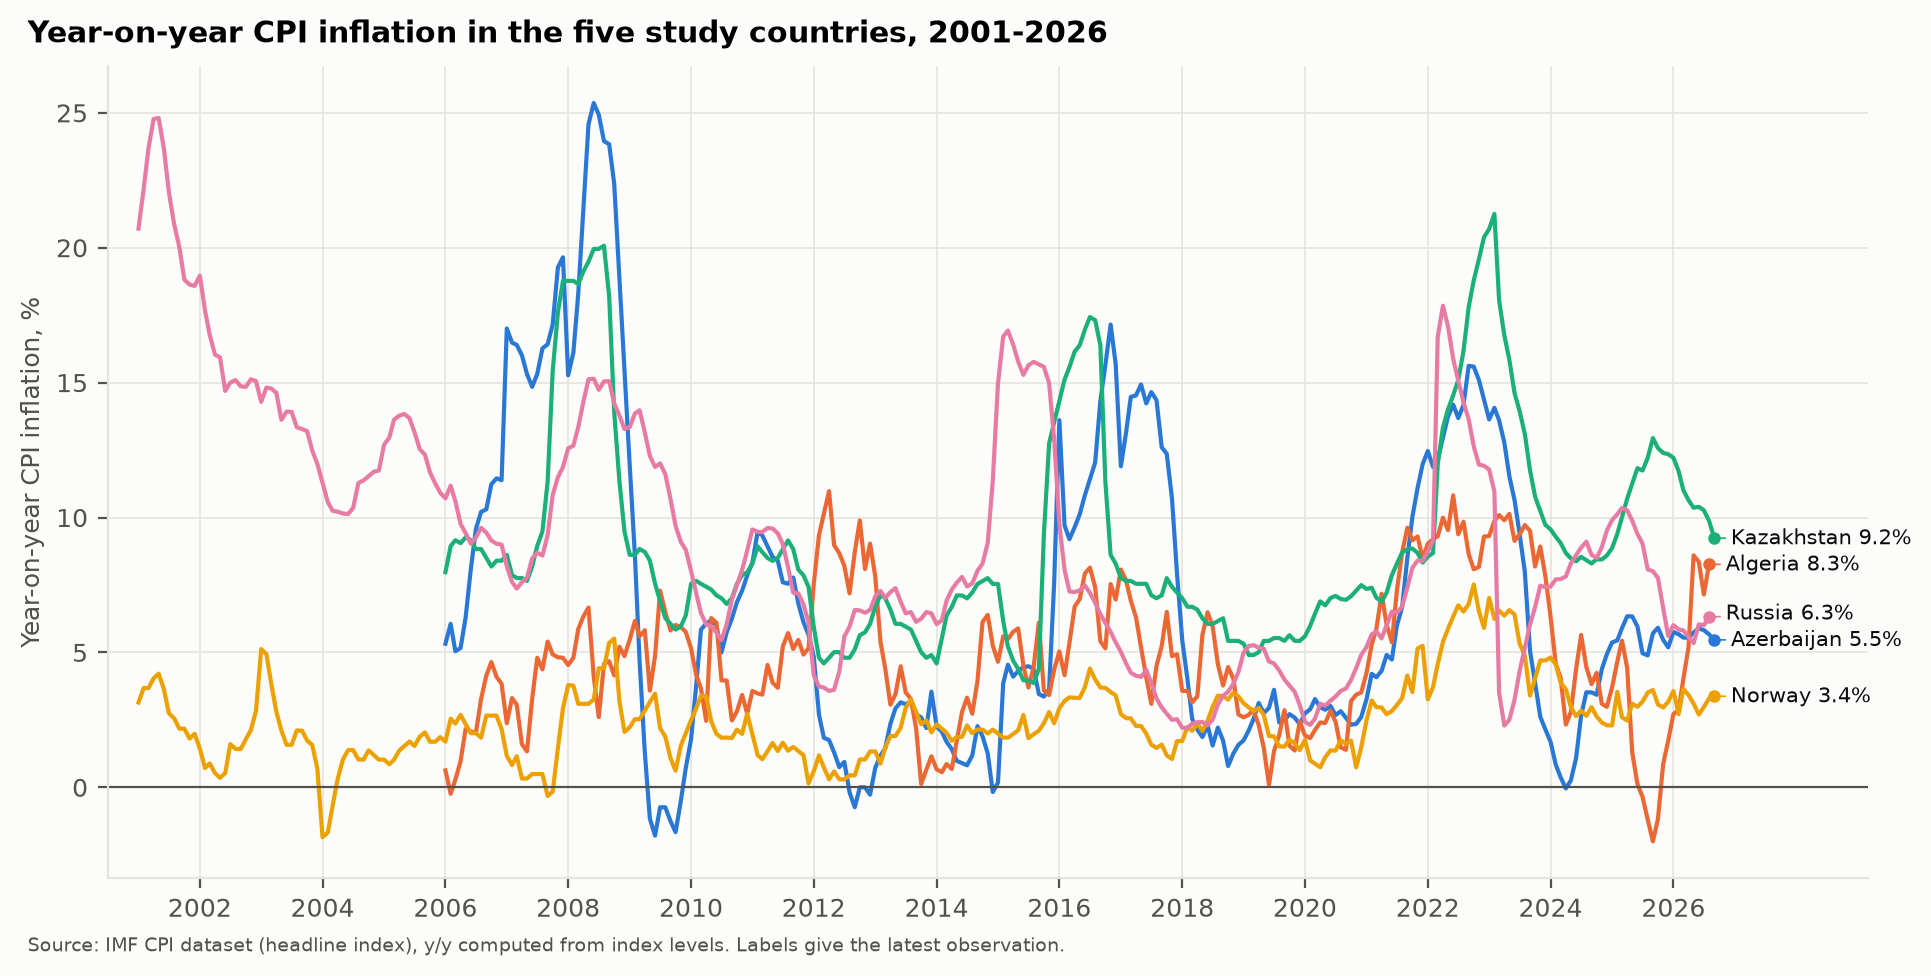
\includegraphics[width=\linewidth]{fig02_inflation_all_countries.png}
\caption{Year-on-year inflation in the comparative countries. The plotted rate is computed within each national headline index; labels refer to the last observation available for each country. Starting dates and ending months differ in this descriptive figure.}
\label{fig:international}
\end{figure}

\begin{figure}[htbp]
\centering
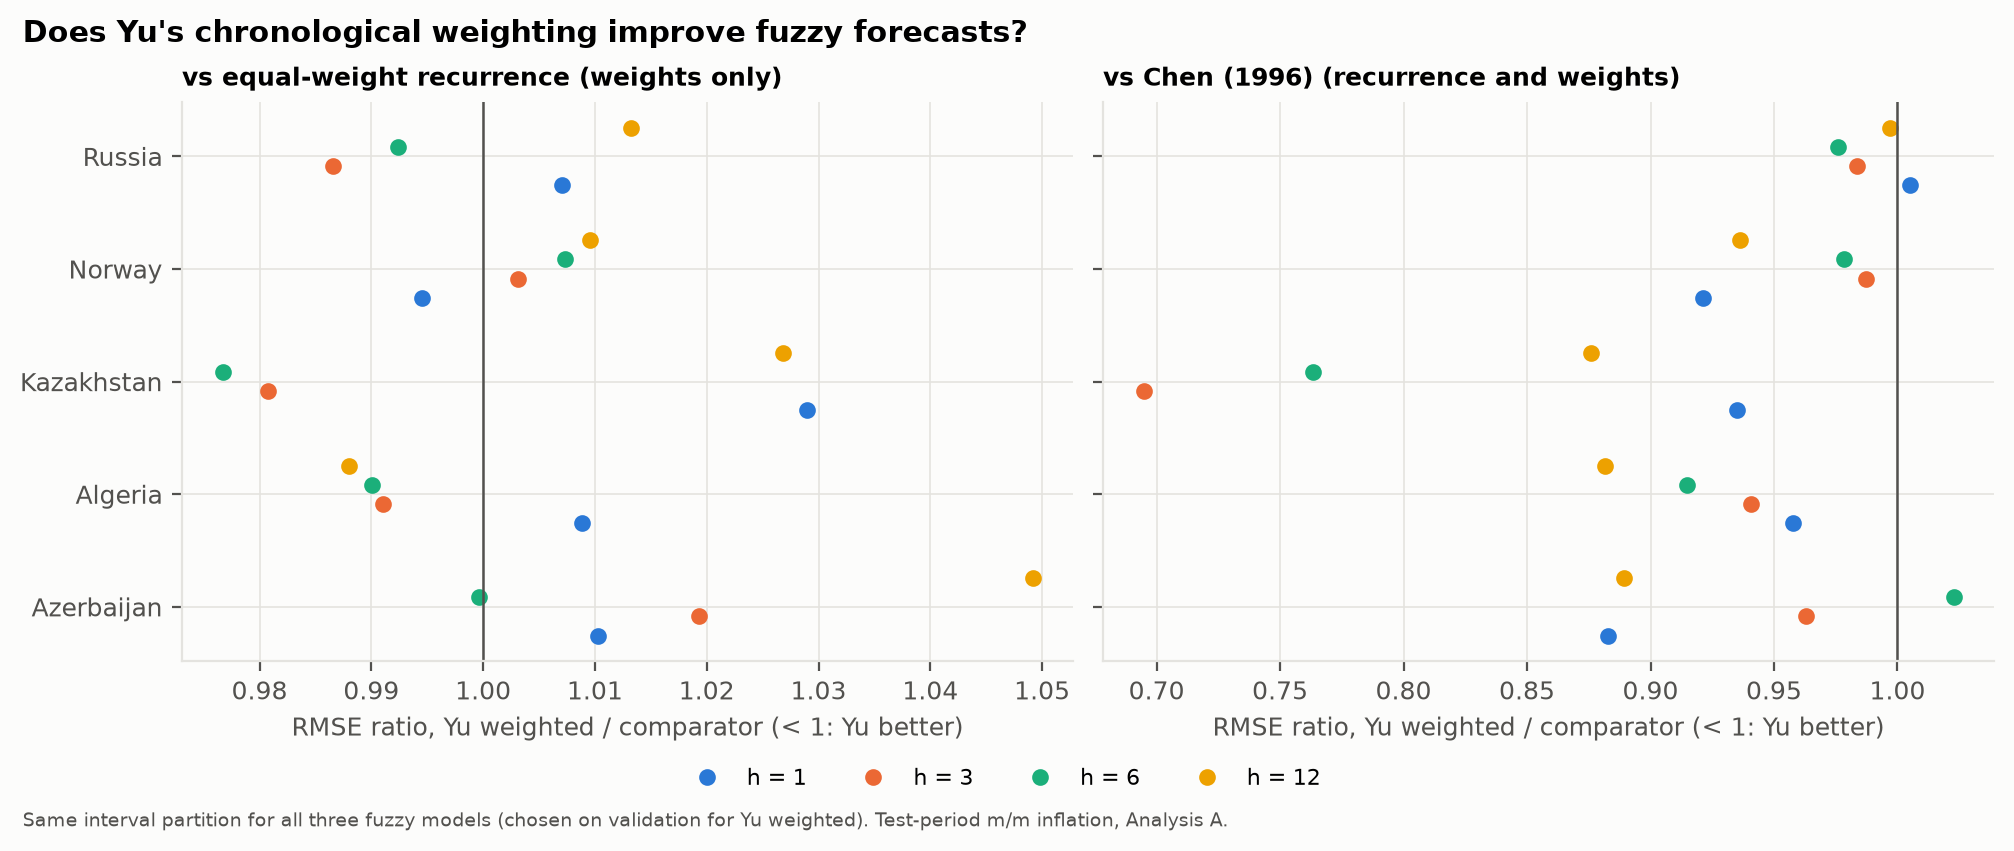
\includegraphics[width=\linewidth]{fig06_yu_weighted_vs_unweighted.png}
\caption{Fuzzy model comparisons holding the interval partition fixed. Ratios below one favor chronological weighting. The left panel isolates weights while retaining recurrence; the right compares recurrence plus weighting with unique-successor averaging. Counts across country--horizon cells are descriptive and not independent replications.}
\label{fig:fuzzy}
\end{figure}

The results in Figure~\ref{fig:fuzzy} do not show a consistent additional gain from the chronological weights. The raw weighted-model advantage over unique-successor averaging is more widespread, which is consistent with the value of keeping repeated relationships. The international annual-rate robustness check leads to the same caution about claiming a general advantage for fuzzy forecasts. The supplementary autoregressive benchmark is occasionally better than the leading primary model, including some Kazakhstan and Russia horizons. Consequently, the primary rankings should always be read as rankings within the stated four-method comparison.

Mean squared loss is dominated by large forecast errors in volatile episodes. The pooled common-period exercise first averages paired loss differences across countries at each origin and then applies the horizon-adjusted test to that monthly sequence. It does not treat five-country observations as five times as many independent months. The twenty country--horizon point rankings likewise share countries and overlapping outcomes, so sign-count probabilities are not treated as confirmatory evidence.

With directly modelled annual inflation, selected ETS forecasts in Azerbaijan, Algeria, and Kazakhstan nearly reproduce the random walk because their smoothing parameter is close to one. This uses a different target and benchmark from the primary monthly-rate experiment.

\section{Pilot survey profiles and sensitivity}
\label{app:survey}

Table~\ref{tab:surveysummary} distinguishes shares, income burdens, and constructed exposure. The national HBS comparison is contextual: the pilot's fourteen recorded categories do not match all official divisions item for item. A low recorded food share may reflect selection, a larger education share, or reporting of irregular expenses as well as underlying consumption differences.

\begin{table}[htbp]
\centering\small
\caption{Pilot survey means under alternative sample definitions.}
\label{tab:surveysummary}
\begin{tabular}{@{}lrrrrrr@{}}
\toprule
Sample & $n$ & Food & Education & March 2026 & 2020--2023 & Spending/income \\
\midrule
Full & 32 & 21.63 & 13.02 & 5.42 & 26.05 & 393.36 \\
Quality-controlled & 26 & 23.85 & 14.01 & 5.42 & 26.22 & 82.84 \\
Consistency subgroup & 25 & 24.16 & 13.41 & 5.41 & 26.24 & 67.90 \\
\bottomrule
\end{tabular}
\par\smallskip
\begin{minipage}{\linewidth}\footnotesize Food and education are percentages of recorded spending. The two exposure columns are percentage increases in basket cost, with the 2020--2023 window counterfactual. Spending/income is a percentage using bracket-midpoint income (lower bound for the open upper bracket). Survey food-at-home spending is not perfectly matched to official CP01.\end{minipage}
\end{table}

\begin{figure}[htbp]
\centering
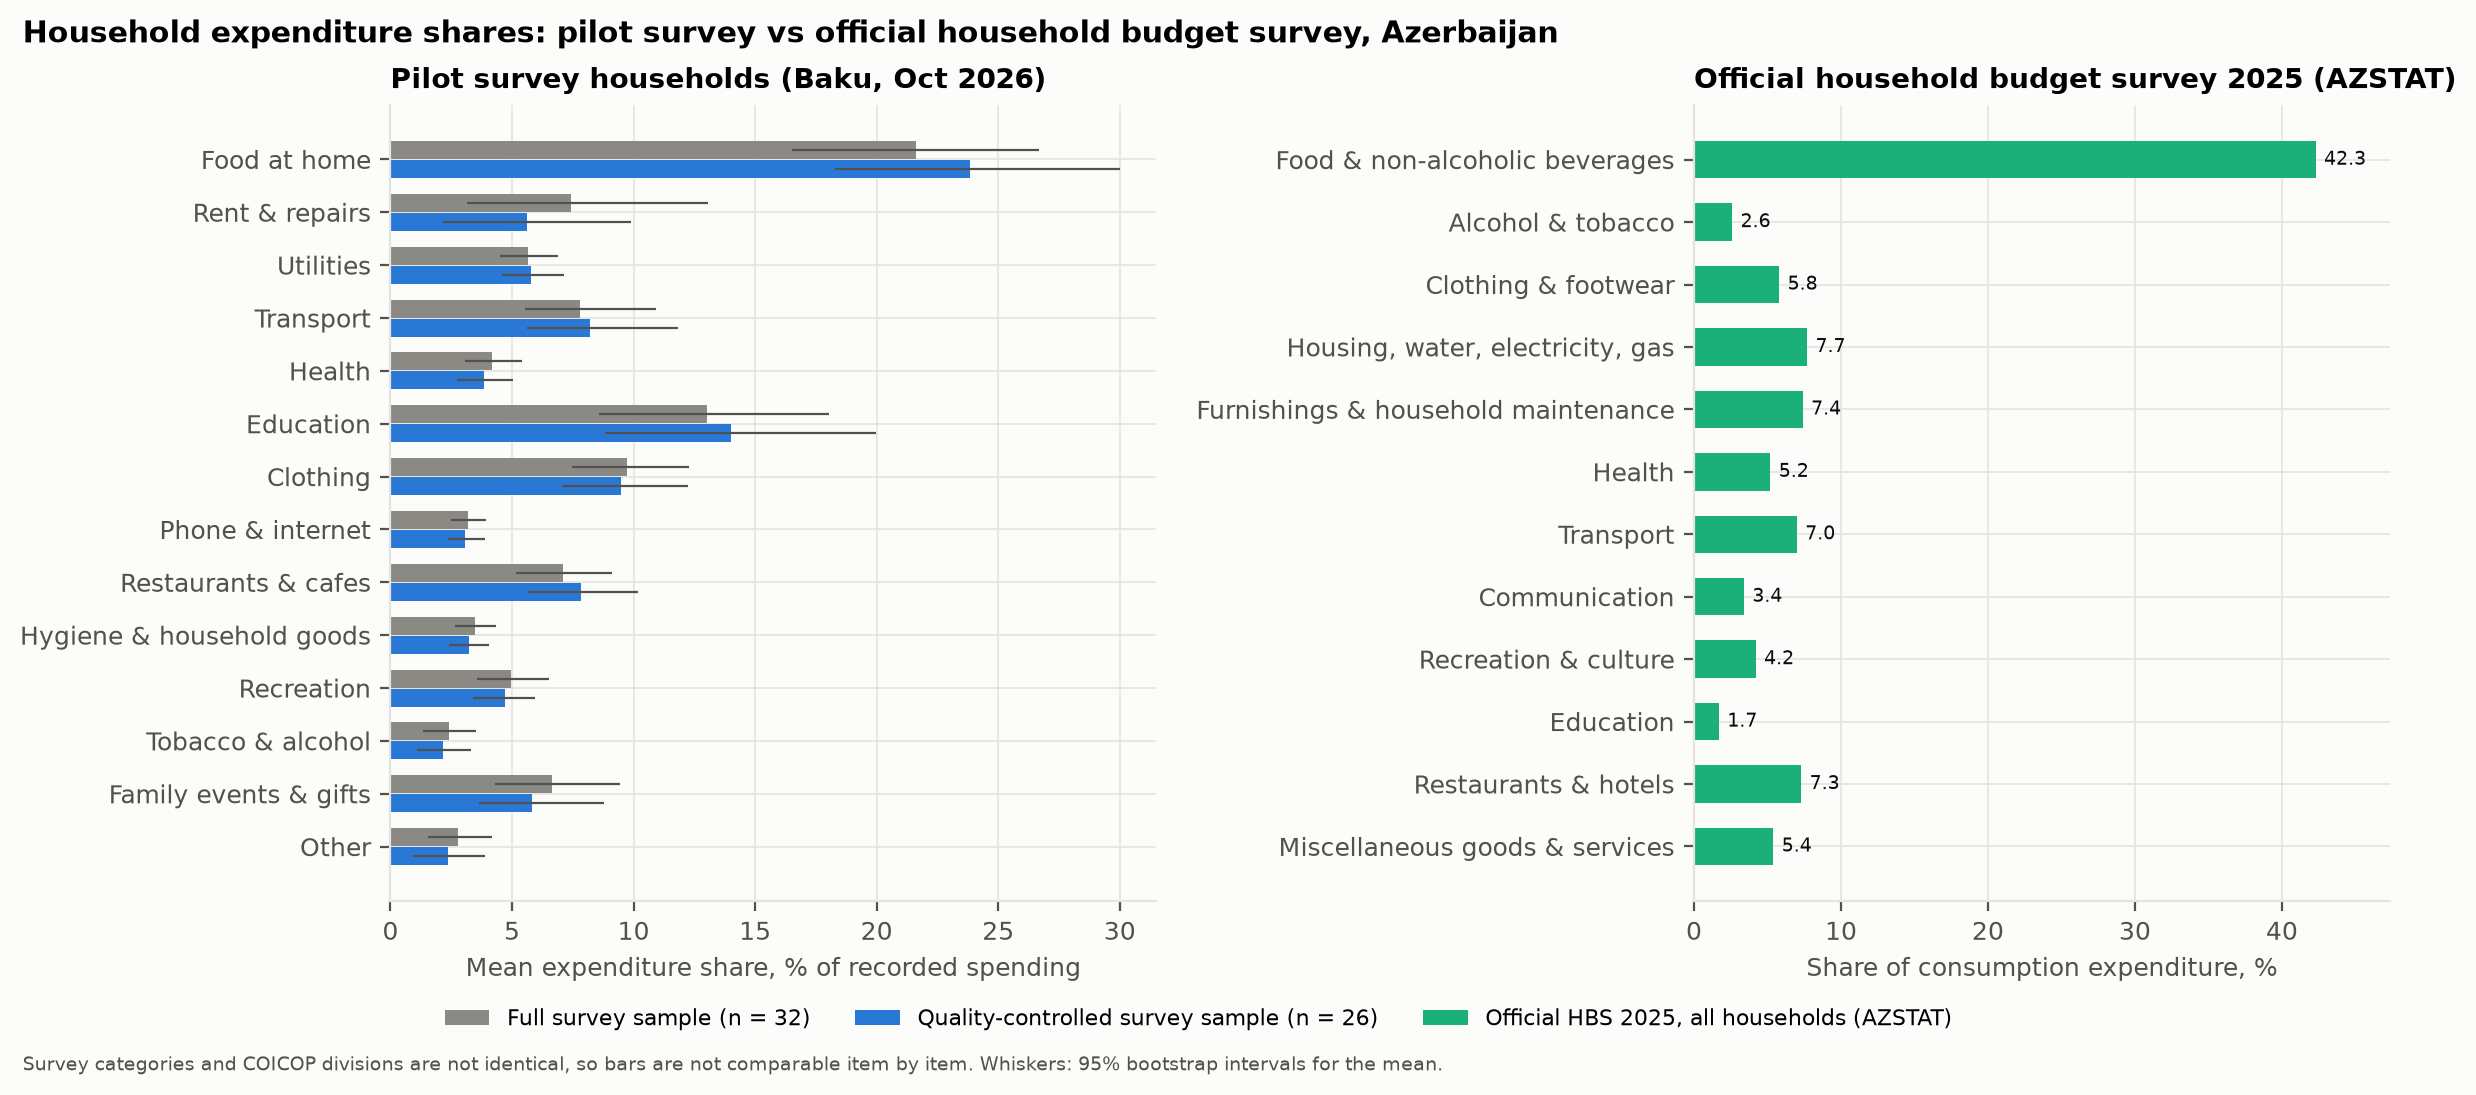
\includegraphics[width=\linewidth]{fig07_household_expenditure_shares.png}
\caption{Pilot spending profiles and the official national expenditure structure. The pilot is a Baku convenience sample; its categories differ from the official COICOP-aligned profile. Whiskers describe bootstrap uncertainty of the sample mean and do not correct selection bias.}
\label{fig:surveyshares}
\end{figure}

\begin{figure}[htbp]
\centering
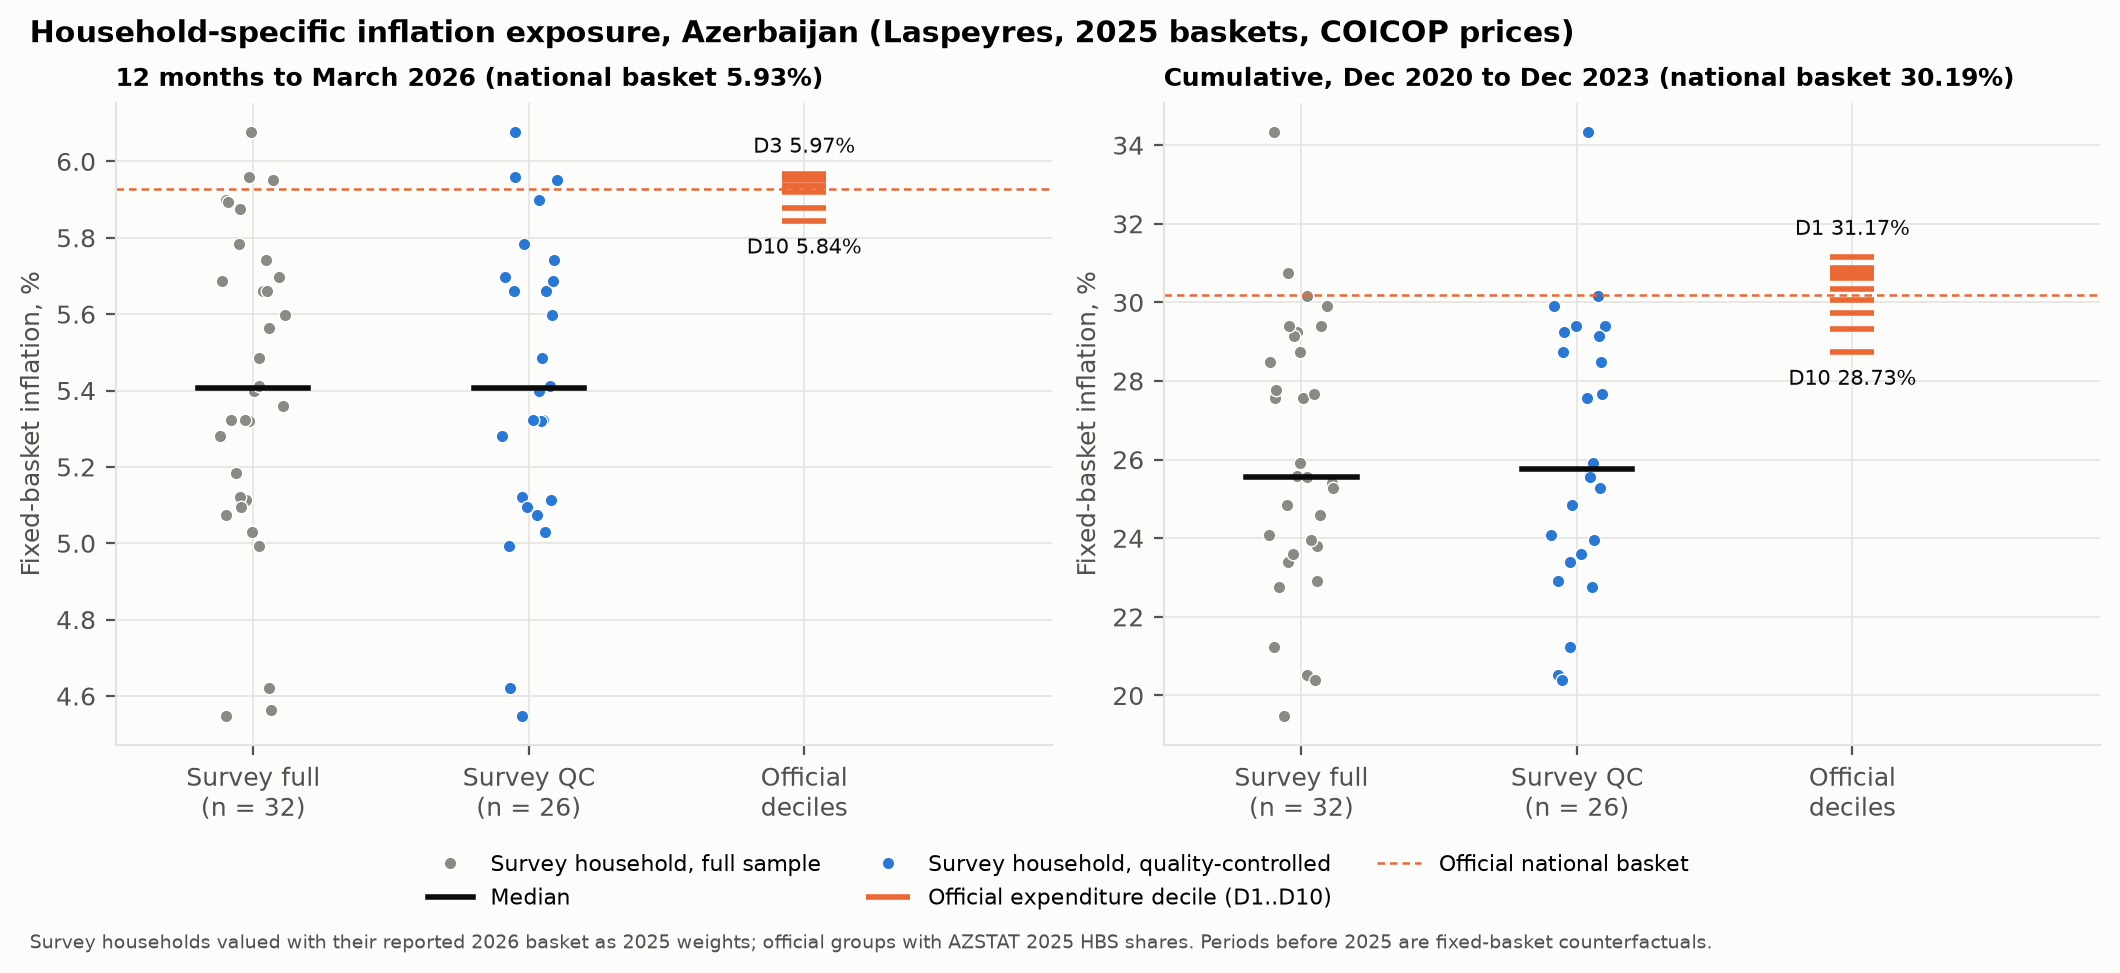
\includegraphics[width=\linewidth]{fig09_household_inflation_exposure.png}
\caption{Constructed household exposure in the pilot and official expenditure-decile baskets. Survey households use their October 2026 reported spending under the fixed 2025 normalization. Earlier windows are counterfactual. The national reference is HBS-weighted basket inflation, not the official CPI.}
\label{fig:surveydistribution}
\end{figure}

\begin{figure}[htbp]
\centering
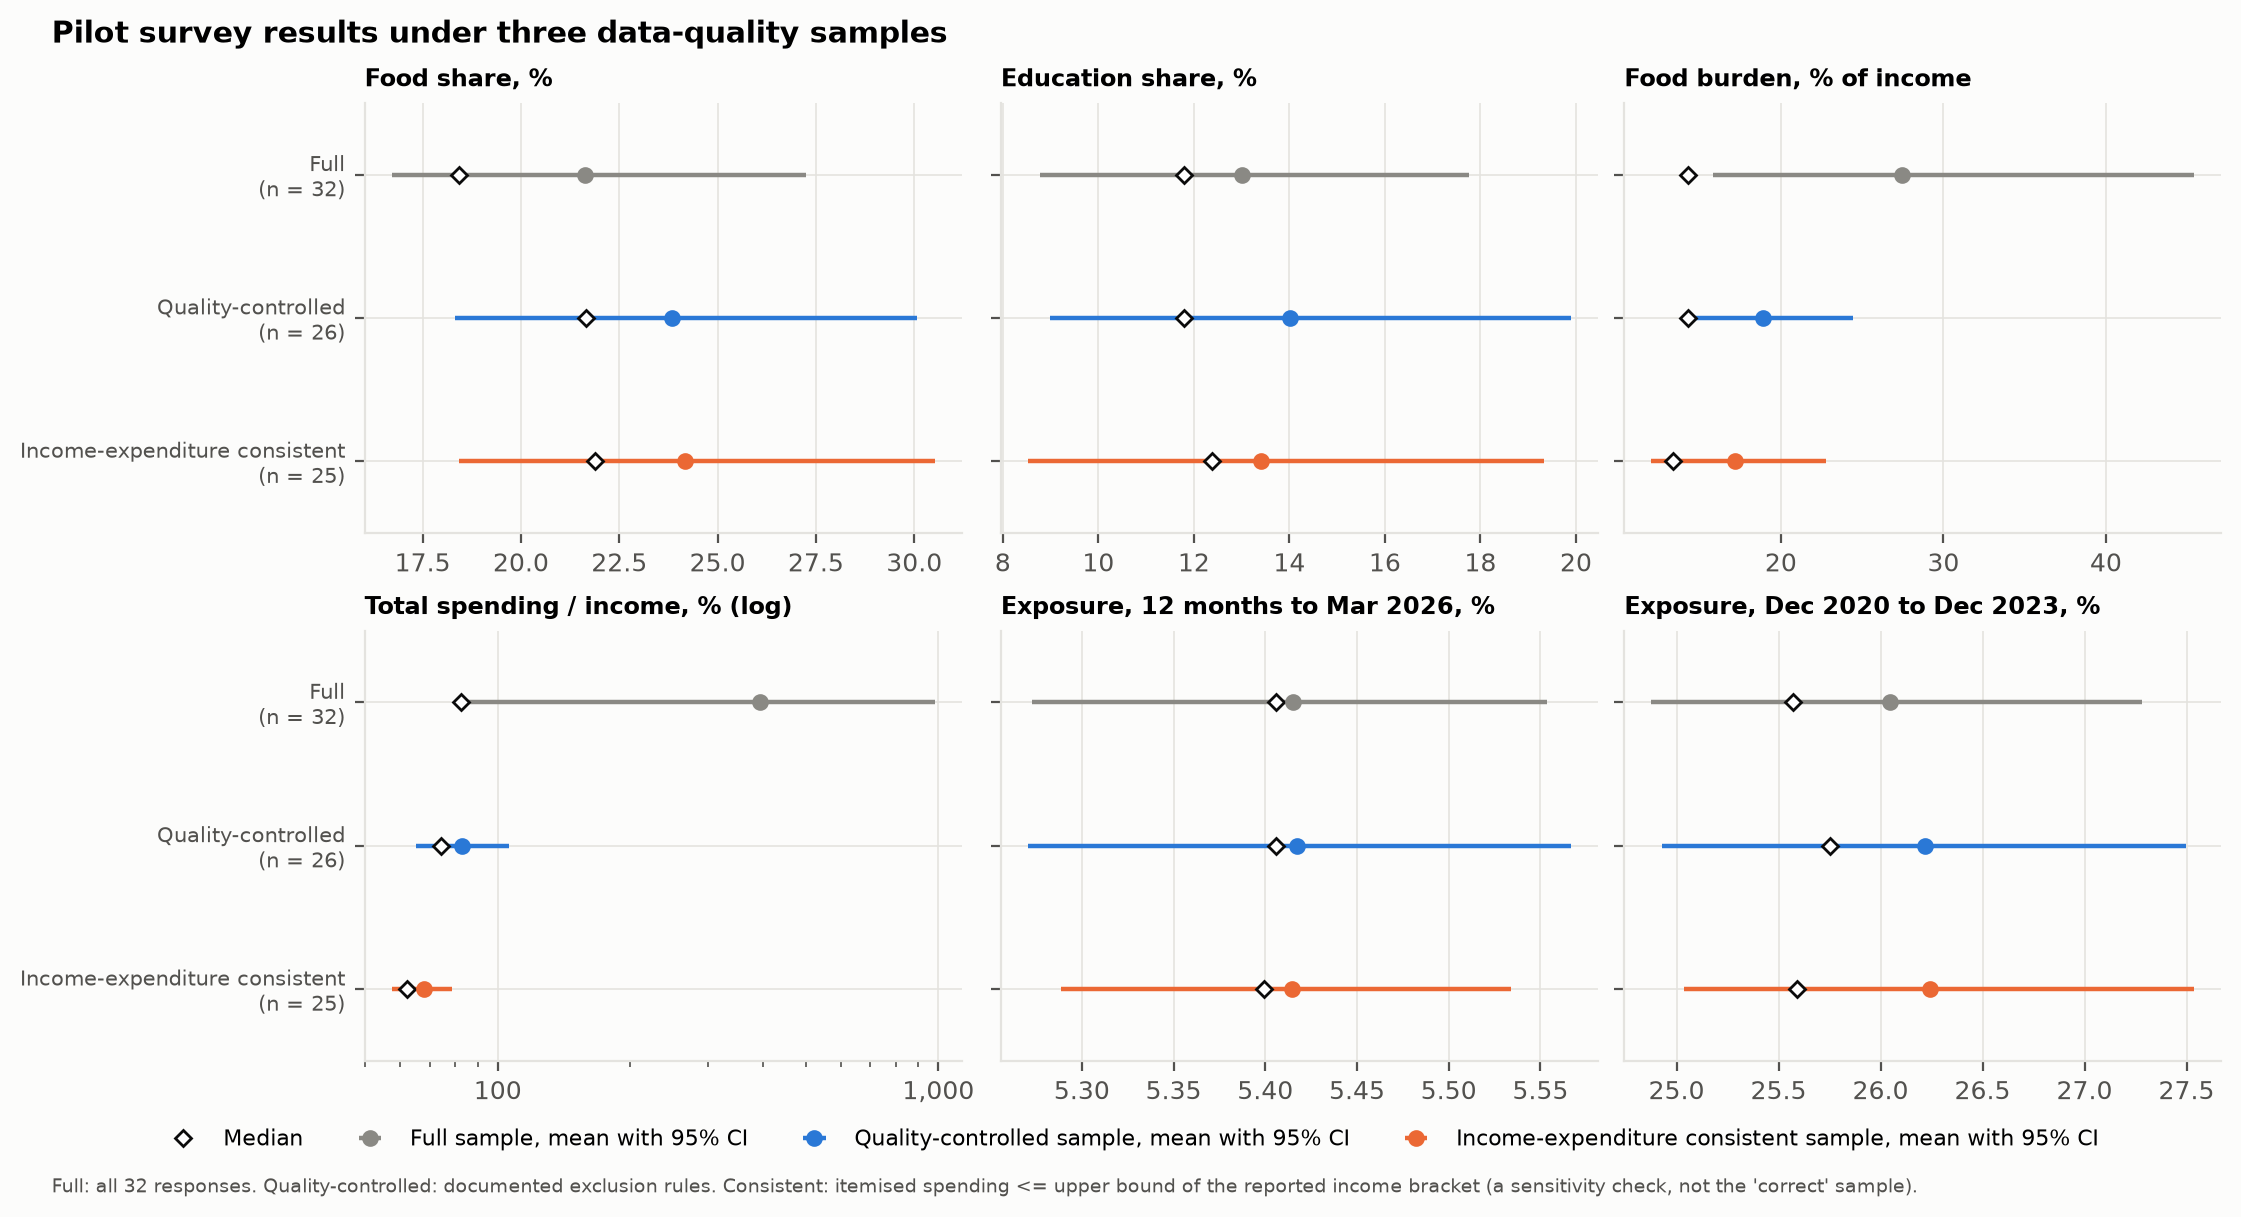
\includegraphics[width=\linewidth]{fig10_survey_sample_sensitivity.png}
\caption{Sensitivity to survey sample rules. Full sample: 32 households; quality-controlled: 26; income--expenditure consistency subgroup: 25. Means and medians are more stable for normalized basket exposure than for spending relative to bracket-midpoint income. The consistency subgroup is a sensitivity sample rather than a population estimate.}
\label{fig:surveysensitivity}
\end{figure}

The survey comparisons in Figures~\ref{fig:surveyshares}--\ref{fig:surveysensitivity} show that data quality affects different quantities differently. The reported income denominator makes income burdens sensitive to bracket assumptions and extreme spending records. Normalizing a household's category amounts into shares removes common scale errors, although it does not remove category-specific recall error. The stable mean exposure across samples therefore establishes a limited robustness result, rather than validating every survey response.

\section{Kazakhstan consumption and geographical exposure}
\label{app:kazakhstan}

Figure~\ref{fig:kazstructure} places the mapped 2025 basket in its published consumption history. Food goods in the stacked panel include alcohol, tobacco, and eating out, whereas the line panel isolates food and non-alcoholic beverages. These measures should not be interchanged. The quarterly 2026 observations are identified separately because they are not full-year averages.

\begin{figure}[htbp]
\centering
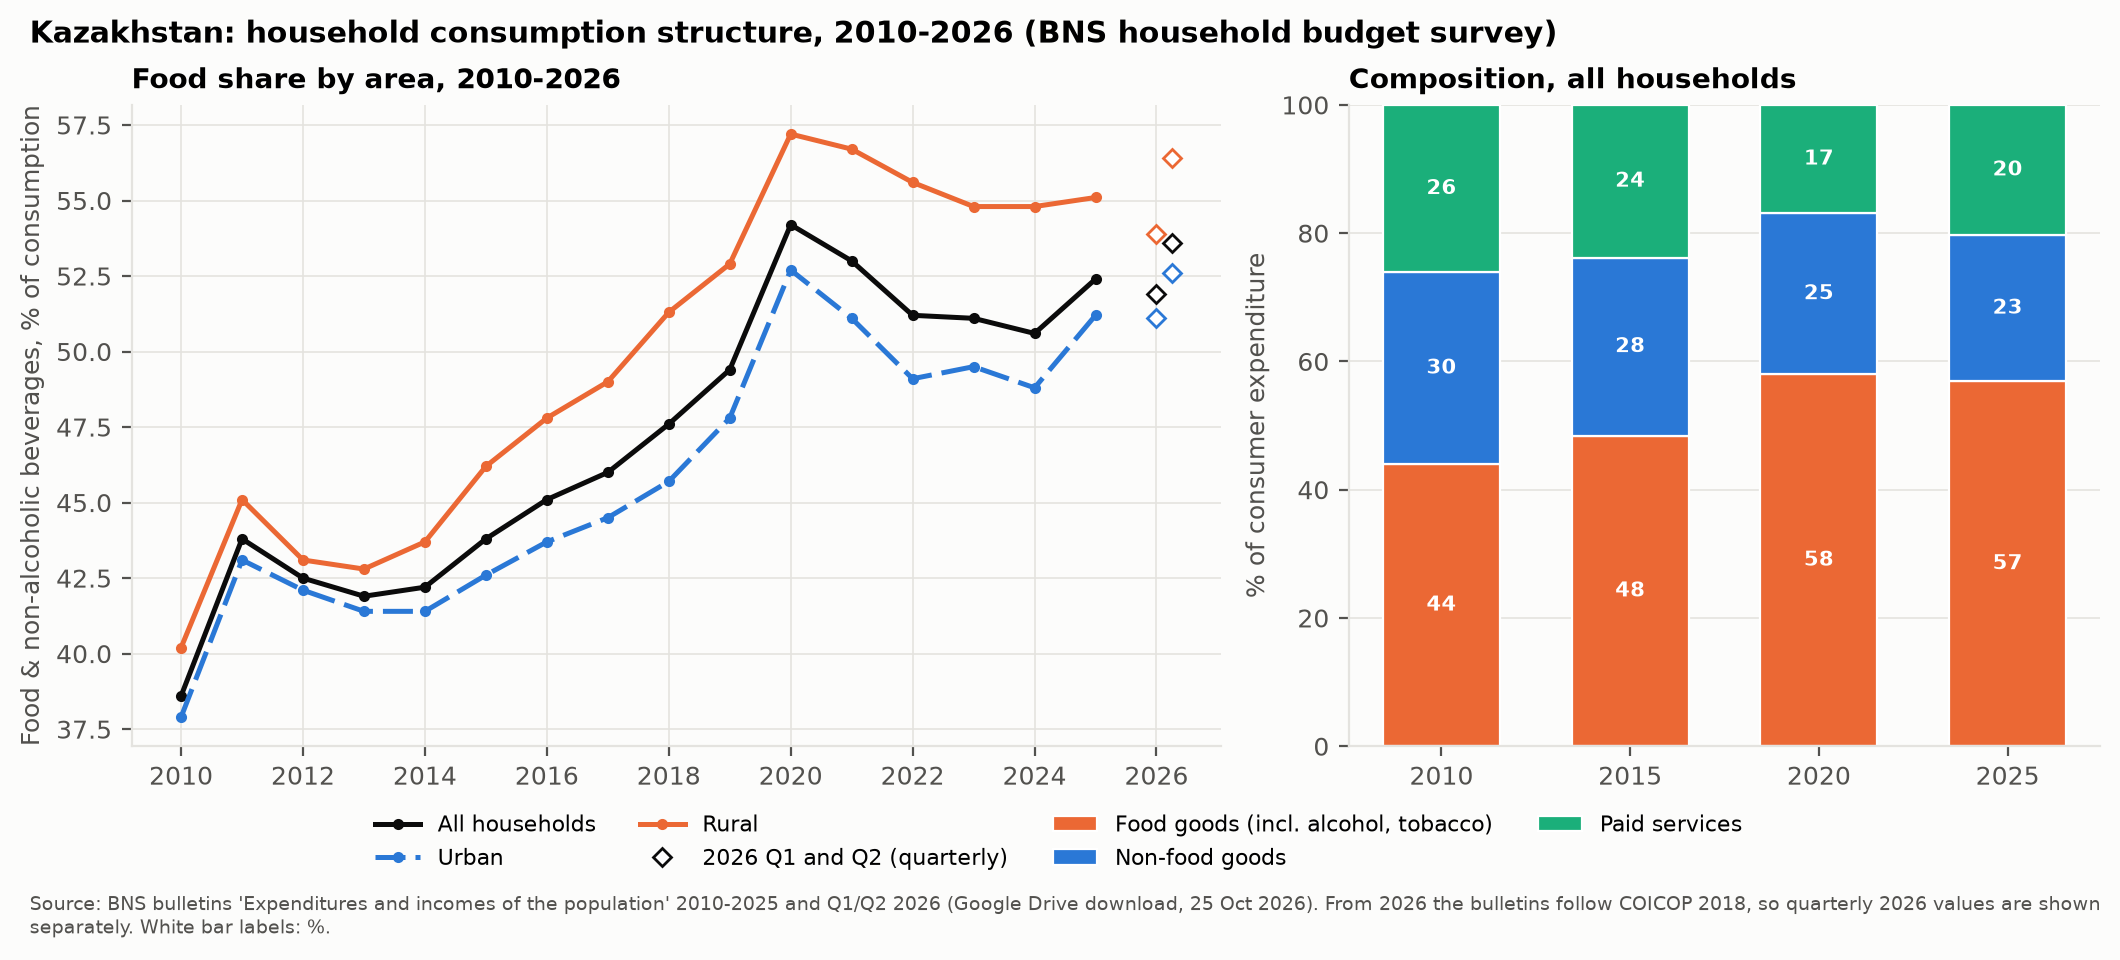
\includegraphics[width=0.94\linewidth]{fig15_kazakhstan_spending_structure.png}
\caption{Kazakhstan consumption structures from BNS household budget bulletins. The line panel reports food and non-alcoholic beverages; the stacked panel reports broader food goods, nonfood goods, and services. Diamonds denote 2026 quarterly observations. Classification changes and period differences limit direct comparisons with annual values.}
\label{fig:kazstructure}
\end{figure}

\begin{figure}[htbp]
\centering
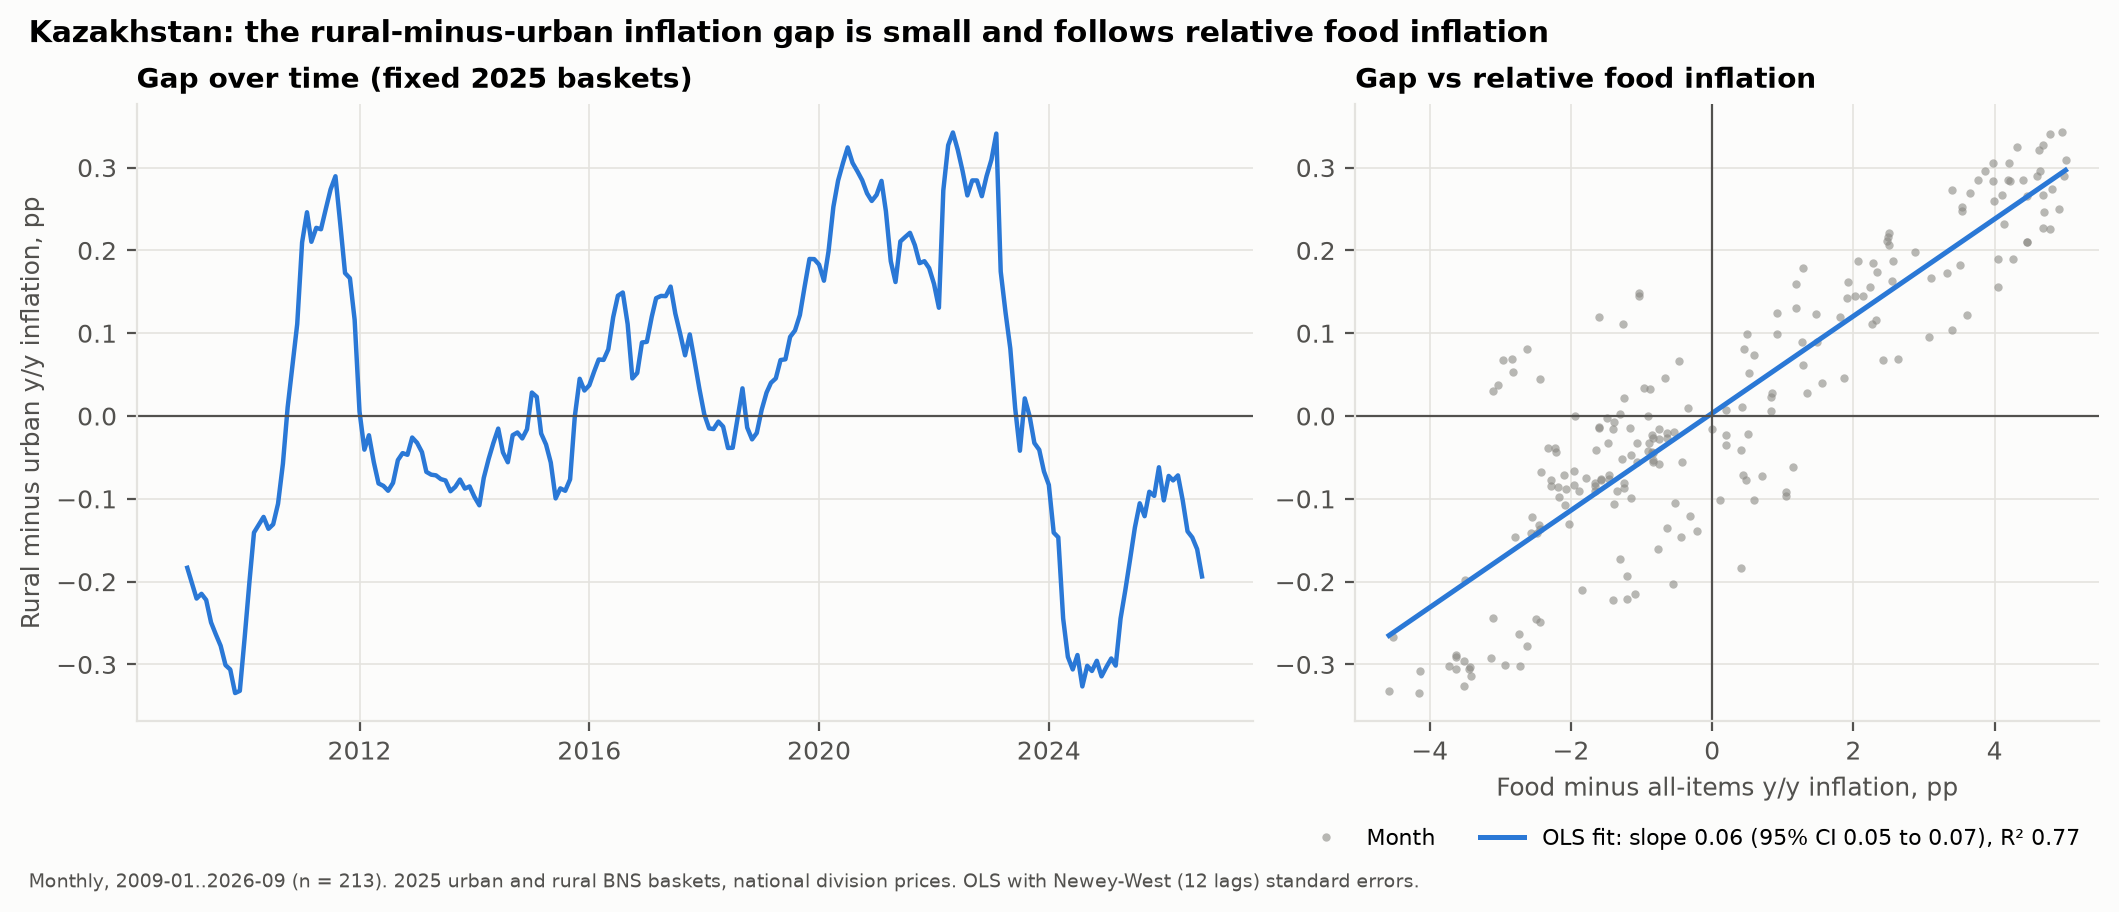
\includegraphics[width=0.94\linewidth]{fig17_kazakhstan_rural_urban_gap.png}
\caption{Kazakhstan's rural-minus-urban annual inflation gap under fixed 2025 baskets, January 2009--September 2026. National division prices are used for both groups. The regression summarizes a shared-price accounting association, with Newey--West standard errors, rather than a causal response or an independent test of forecast performance.}
\label{fig:kazgap}
\end{figure}

The 213 observations in Figure~\ref{fig:kazgap} give a slope of approximately 0.06 on relative food inflation (Newey--West 95\% interval 0.05--0.07; $R^2=0.77$). Comparing it with Azerbaijan's decile slope cannot rank distributional inequality: geographical groups and expenditure deciles partition households differently.

\end{document}
